% !TeX spellcheck = de_DE

\chapter{Spezifikation}
\label{chap:spezi}

Nachdem im Projektplan die Rahmenbedingungen und zeitlichen Abläufe formal festhalten wurden, werden nun in der Spezifikation, die Anforderungen an den, während des Projekts \profire, zu entwickelnde Prototyp erfasst.

\section{Einleitung}

\subsection{Zweck der Spezifikation}
Die in der Analyse gesammelten Anforderungen an die \hyperlink{tab:anwendung}{Software} müssen in der Spezifikation geordnet und schriftlich festgehalten werden.
Des Weiteren ist die Spezifikation Grundlage für alle weiteren entstehenden Dokumente und entscheidet im Streitfall darüber, ob das Resultat den Abmachungen und Anforderungen des Kunden und den Betreuern an die \hyperlink{tab:anwendung}{Software} entspricht.
Außerdem ist die Spezifikation notwendig für den Entwurf, die Implementierung, die Testvorbereitung, die Prüfung und die Abnahme.

Das Team verpflichtet sich, die Spezifikation aktuell zu halten und mit anderen Dokumenten abzustimmen.

Auch nach der Auslieferung soll die Spezifikation anderen Entwicklern das Einarbeiten, Verbessern, Erweitern und die Wartung der \hyperlink{tab:anwendung}{Software} erleichtern.

\subsection{Lesekreis der Spezifikation}
Folgende Personen gehören zum Leserkreis der Spezifikation:
\begin{itemize}
	\item Der Kunde
	\item Das gesamte Entwicklerteam
	\item Die universitären Betreuer
\end{itemize}

\subsection{Einsatzbereich und Ziele von ProFire}
Die \hyperlink{tab:anwendung}{Software} wird im Rahmen des Studienprojekts 2015/2016 an der Universität Stuttgart für das Institut für Visualisierung und Interaktion entwickelt.

\profire soll Feuerwehrleute bei ihren Einsätzen unterstützen.
Insbesondere dann, wenn diese sich nicht mehr auf ihre normale visuelle Wahrnehmung verlassen können.
In solchen Situationen verwenden Feuerwehrleute häufig Wärmebildkameras.
Hierbei entsteht jedoch das Problem der \hyperlink{tab:strahlung}{ÜberÜberstrahlung} und der fehlenden dreidimensionalen Wahrnehmung (\va Einschätzung von Distanzen).
Diese Probleme sollen mit diesem Projekt angegangen und behoben werden.

Dazu wird ein Prototyp, bestehend aus einer Wärmebildkamera, \hyperlink{tab:tiefe}{Tiefenbild}kamera, Halterung, Ausgabemodul und der passenden \hyperlink{tab:anwendung}{Software} dazu, entwickelt.
Die \hyperlink{tab:anwendung}{Software} soll die Bilder dieser beiden Kameras so überlagern, sodass man Kanten des überstrahlten Objektes nachzeichnen kann und Entfernungen bestimmen kann.
Es sollen die positiven Eigenschaften beider Kameras ausgenutzt werden, um Schwächen der einen mit Hilfe der Stärken der anderen zu reduzieren.

Das Projekt wurde von Prof. Dr. Schmidt vom Institut für Visualisierung und Interaktive Systeme der Universität Stuttgart initiiert.

\subsection{Überblick über den Aufbau der Spezifikation}
\begin{description}
	\item[\cref{chap:spezi_desc} -- \nameref{chap:spezi_desc}] Gibt einen Ausblick über den Umfang dieser \hyperlink{tab:anwendung}{Software}. Es werden  außerdem Informationen über die Funktionen der \hyperlink{tab:anwendung}{Software} geklärt.
	\item[\cref{chap:spezi_req} -- \nameref{chap:spezi_req}] Zeigt alle Anforderungen von \profire auf. Diese werden in nicht-funktionale und funktionale Anforderungen aufgeteilt.
	\item[\cref{chap:spezi_setup} -- \nameref{chap:spezi_setup}] Beschreibt den Prototypaufbau und die Oberfläche (mithilfe eins UI-Prototyps).
	\item[\cref{chap:spezi_usecases} -- \nameref{chap:spezi_usecases}] Gibt einen Überblick über alle möglichen Anwendungsfälle dieser \hyperlink{tab:anwendung}{Software}.
	\item[\cref{chap:spezi_append} -- \nameref{chap:spezi_append}] Hier findet man das Begriffslexikon.
	\item[\cref{chap:spezi_version} -- \nameref{chap:spezi_version}] Dieses Kapitel beinhaltet die Versionshistorie dieser Spezifikation.
\end{description}

\subsection{Verwendete Abkürzungen und Schreibweisen}
Alle für das Projekt relevanten Fachbegriffe und Abkürzungen sind im Begriffslexikon 
(am Ende dieses Dokuments) aufgeführt.

\subsection{Aufbau dieses Dokuments}
Neben der allgemeinen Beschreibung des \hyperlink{tab:system}{System}s, sollen die Profile aller späteren Nutzer des \hyperlink{tab:system}{System} skizziert werden.
Darüber hinaus sollen die Anforderungen an die Funktion des \hyperlink{tab:system}{System}s und die geforderten Qualitäten hinsichtlich der \hyperlink{tab:anwendung}{Software} selbst dokumentiert werden.

\section{Allgemeine Beschreibung}
\label{chap:spezi_desc}

\subsection{Einbettung}
Das \hyperlink{tab:system}{System} \profire soll hauptsächlich bei der Feuerwehr genutzt werden.
Das \hyperlink{tab:system}{System} soll in einer Windows-Umgebung (Windows 7 oder neuer) laufen und eine visuelle Ausgabe auf dem ausführenden Laptop, sowie einem im selben WLAN-Netz befindlichen Handy (LG G Flex 2) und einer angeschlossenen Augmented Reality-Brille (\meta), unterstützen.

Für die Funktionalität verwendet das \hyperlink{tab:system}{System} eine Kombination aus Wärmebild- und \hyperlink{tab:tiefe}{Tiefenbild}kamera zur Messung der Daten. Die Auswertung erfolgt dann durch das \hyperlink{tab:system}{System}.

Das .NET Framework Version 4.5 oder neuer, sowie die SDKs der gegebenen Kameras müssen vorhanden sein.

\subsection{Überblick über die Funktionen}
\begin{itemize}
	\item Einbenutzersystem
	\item Halterung als Case für Wärmebildkamera und \hyperlink{tab:tiefe}{Tiefenbild}kamera (sowohl auf Stick als auch am Helm montierbar)
	\item Anzeige auf Augmented-Reality-Brille, Laptop und Smartphone
	\item Anzeige von Informationen wie Temperatur, Entfernung und Kontur von Objekten
	\item Möglichkeit des Wechseln der Anzeigebilder:
	\begin{itemize}
		\item \hyperlink{tab:tiefe}{Tiefenbild}
		\item Wärmebild
		\item RGB-Bild
		\item Generiertes Bild (Wärmebild-\hyperlink{tab:tiefe}{Tiefenbild}-Überlappung)
	\end{itemize}
\end{itemize}

Weitere Einzelheiten und Erläuterungen werden im Abschnitt 3.2 „Funktionale Anforderungen“ beschrieben.

\subsection{Mengengerüst}
Folgende Kenngrößen sind relevant für das \hyperlink{tab:system}{System}:
\begin{itemize}
	\item Es werden Daten aus einer Wärmebild- und \hyperlink{tab:tiefe}{Tiefenbild}kamera verarbeitet.
	\item Das \hyperlink{tab:system}{System} kann mehrfach, aber immer nur von einer Person genutzt werden.
	\item Erkennt Temperaturen im Messbereich in °C durch Wärmebildkamera.
	\item Daten der Wärmebildkamera:
	\begin{itemize}
		\item gemessene Objekt-Temperatur, Anzeige der Temperatur-Zonen in °C 
		\item Temperatur der Wärmebildkamera in °C
		\item Umgebungtemperatur in °C
		\item Emissionkoeffizient zur Bestimmung der Objekt-Temperatur
		\item Geräte-spezifische Konstante
		\item Auflösung von 382*288 Pixel
	\end{itemize}
	\item Erkennt Entfernungen im Messbereich in m (Meter) durch \hyperlink{tab:tiefe}{Tiefenbild}kamera.
	\item Daten der \hyperlink{tab:tiefe}{Tiefenbild}kamera:
	\begin{itemize}
		\item relative Distanz der Objekte in der Umgebung
		\item Auflösung 640*480
	\end{itemize}
\end{itemize}

\subsection{Profil der ProFire-Nutzer}
Die Benutzer der \hyperlink{tab:anwendung}{Software} arbeiten bei der Feuerwehr und haben bereits Erfahrungen mit Wärmebildkameras in der Praxis gesammelt.
Für die Nutzung der \hyperlink{tab:anwendung}{Software} \profire sind keine Programmierkenntnisse in der Sprache C\# (auf welcher \profire basiert) oder anderen Programmiersprachen notwendig.
Daher wird die Nutzung der \hyperlink{tab:anwendung}{Software} auch keine Einschränkungen für den Nutzer haben.

\subsection{Entwicklungswerkzeuge}
\begin{description}
	\item [Eclipse / Visual Studio] --- Entwicklungsumgebung
	\item [GitLab \& Google Drive] --- Konfigurationsmanagement
	\item [\LaTeX{}] --- Dokumentenerstellung
	\item [UmLet] --- UML-Modellierung
	\item [RevAger] --- Review-Organisation und -protokollierung
	\item [Testsuite-Management (TSM)] --- Testfallverwaltung
\end{description}

\subsection{Einschränkungen}
\begin{itemize}
	\item Programmiersprache C\# 5
	\item Verwendung von den Kamera SDKs
	\item Splashtop Personal
	\item optris PI Connect 2.9.2147.0
\end{itemize}

\subsection{Annahmen und Abhängigkeiten}
Bei der Spezifikation wurde von folgenden externen Einflussfaktoren ausgegangen:
\begin{itemize}
	\item Für das Projekt stehen ausreichend Personen zur Verwirklichung des Projekts zur Verfügung.
	\item Die \hyperlink{tab:anwendung}{Software} soll nach der ersten Inbetriebnahme solange wie möglich bestehen bleiben, da sie voraussichtlich nicht durch ein Nachfolgesystem ersetzt wird.
	Es ist aber nicht ausgeschlossen, dass in Zukunft neue Funktionen in das bestehende \hyperlink{tab:system}{System} eingepflegt werden.
\end{itemize}

\section{Einzelanforderungen}
\label{chap:spezi_req}

\subsection{Nichtfunktionale Anforderungen}

\subsubsection{Auflösung}
Die auf die Brille projizierten Bildern können mit einer  Auflösung von mindestens 960*540 angezeigt werden.
Ziel ist es dadurch die Realität zu ergänzen, ohne die Wahrnehmung der Umgebung zu verhindern.
Die genaue Auflösung und Anzeige wird während der Entwicklung noch optimiert.

\subsubsection{Bedienbarkeit}
Die Bedienbarkeit der \hyperlink{tab:anwendung}{Software} soll intuitiv sein.
Der User kann zwischen der Ausgabe von dem Wärmebild, \hyperlink{tab:tiefe}{Tiefenbild}, RGB-Bild und der Fusion wechseln, indem er einen Schalter betätigt (Im Prototyp eine Maus, später eventuell durch Gesten die von der Brille wahrgenommen werden).
Bei der Maus werden lediglich die Tasten benötigt.

\subsubsection{Wartbarkeit / Erweiterbarkeit}
Die \hyperlink{tab:anwendung}{Software} wird zurzeit noch als Prototyp entwickelt, deshalb werden als Priorität die Projektion der Wärme- und \hyperlink{tab:tiefe}{Tiefenbilder} gesetzt.
Die Schnittstelle wird dennoch so implementiert, das später weiter Module eingebettet werden können.

\subsubsection{Ausfallsicherheit}
Da die \hyperlink{tab:anwendung}{Software} zurzeit noch als Prototyp entwickelt wird soll die Ausfallsicherheit der \hyperlink{tab:anwendung}{Anwendung} so sicher sein, dass sie Tests in nach simulierten Testumgebungen standhält.
Das heißt sie sollte mindestens eine halbe Stunde ohne Probleme laufen können.
Die  \hyperlink{tab:anwendung}{Software} muss nicht gegen hardwareseitige Abstürzte, wie Crash der verwendeten SDKs oder Entfernen einer Kamera, unempfindlich sein.
Dennoch wird eine höhere Ausfallsicherheit angestrebt.

\subsection{Funktionale Anforderungen}

\subsubsection{Anzeigen von Temperatur und Distanz}
Ziel der \hyperlink{tab:anwendung}{Anwendung} ist es mehr Informationen über die Umgebung zu bekommen, \va die Distanz zu Objekten und die Temperatur sollen angezeigt werden.
Um dies zu erreichen, wird die Temperatur und Distanz vom Mittelpunkt des Bildes, welches durch ein Fadenkreuz festgelegt wird, am rechten oberen Bildrand in allen verschieden Kameramodi angezeigt.

\subsubsection{RGB-Bildanzeige}
Die Anforderung der Projektion des RGB Bildes auf der Brille ohne weitere Informationen macht für den Endbenutzer Sinn, da er durch die Kamera in das Bild hineinzoomen kann.
Zusätzlich ermöglicht die Kameraführung mit Hand dem User um die Ecke zu sehen, oder vor \bzw hinter Hindernissen die Lage aufzunehmen.

\subsubsection{Tiefenbildanzeige}
Um mehr Informationen über die Umgebung zu bekommen, kann man durch die \hyperlink{tab:tiefe}{Tiefenbildanzeige} einen räumlichen Eindruck erreichen.
Die \hyperlink{tab:tiefe}{Tiefenbildanzeige} soll zuverlässig bei einer Reichweite von 0.5m bis 5m die \hyperlink{tab:tiefe}{Tiefe} des Bildes anzeigen.
Das \hyperlink{tab:tiefe}{Tiefenbild} ist zuverlässig innerhalb von Umgebungen, welche nicht von  \hyperlink{tab:sonne}{Sdirekter Sonnenbestrahlung} betroffen sind.
Zusätzlich wird das \hyperlink{tab:tiefe}{Tiefenbild} auch bei Dunkelheit zuverlässig angezeigt.

\subsubsection{Wärmebildanzeige}
Durch Anzeige des Wärmebildes kann der User die Objekte im Raum anhand deren Temperatur wahrnehmen.
Da verschiedene Temperaturen einem Farbspektrum entsprechen, kann der User die verschiedene Temperaturen von Objekten und des Raumes wahrnehmen.
Die Wärmebildkamera ignoriert, im Gegensatz zur \hyperlink{tab:tiefe}{Tiefenbild}kamera, \hyperlink{tab:sonne}{Sonne}, Rauch und Lichtverhältnisse.
Problematisch dagegen sind Metallflächen, Spiegel und Glasscheiben.

\subsubsection{Generiertesbild (Wärmebild-Tiefenbild-Überlappung)}
Mit Ziel der besseren Konturenerkennung von reflektierenden / \hyperlink{tab:strahlung}{abstrahlenden} / in-einderliegenden Gegenständen für den User zu rendern.
Das Bild das der User am Ende bekommt, soll eine Fusion des Wärmebildes und \hyperlink{tab:tiefe}{Tiefe}nbilds sein, mit schärferen Konturen und Kanten.
Ziel ist es das Wärmebild genauer und schärfer zu machen.

\subsubsection{Zuverlässige Daten in Echtzeit}
Die \hyperlink{tab:anwendung}{Anwendung} ist für den Gebrauch in Echtzeit bestimmt und muss daher die Temperatur und Distanz ohne Verzögerungen anzeigen können.

\subsubsection{Wahl der Ausgabemethode}
Der Nutzer soll die Möglichkeit haben, eine Ausgabe auf der Brille zu verhindern.
In diesem Fall, wird das mobile Anzeigegerät als einzige Ausgabemethode verwendet.
Um dies zu erreichen, soll die Möglichkeit bestehen, auf der kompletten Brille ein schwarzes Overlay anzuzeigen.
Dies hat die Wirkung, dass die Ausgabe für den Nutzer transparent erscheint.

\section{\setup}
\label{chap:spezi_setup}

Der schematische Aufbau soll wie in \cref{fig:spezi_halterung} dargestellt aussehen, dabei trägt der Anwender einen Rucksack in dem ein Laptop enthalten ist.
Beide Kameras sind dauerhaft mit dem Laptop verbunden.
Zusätzlich trägt der Nutzer die \meta Brille.
\begin{figure}[b]
	\centering
	\begin{subfigure}[t]{0.45\textwidth}
		\centering
		\ifthenelse{\boolean{jpg}}{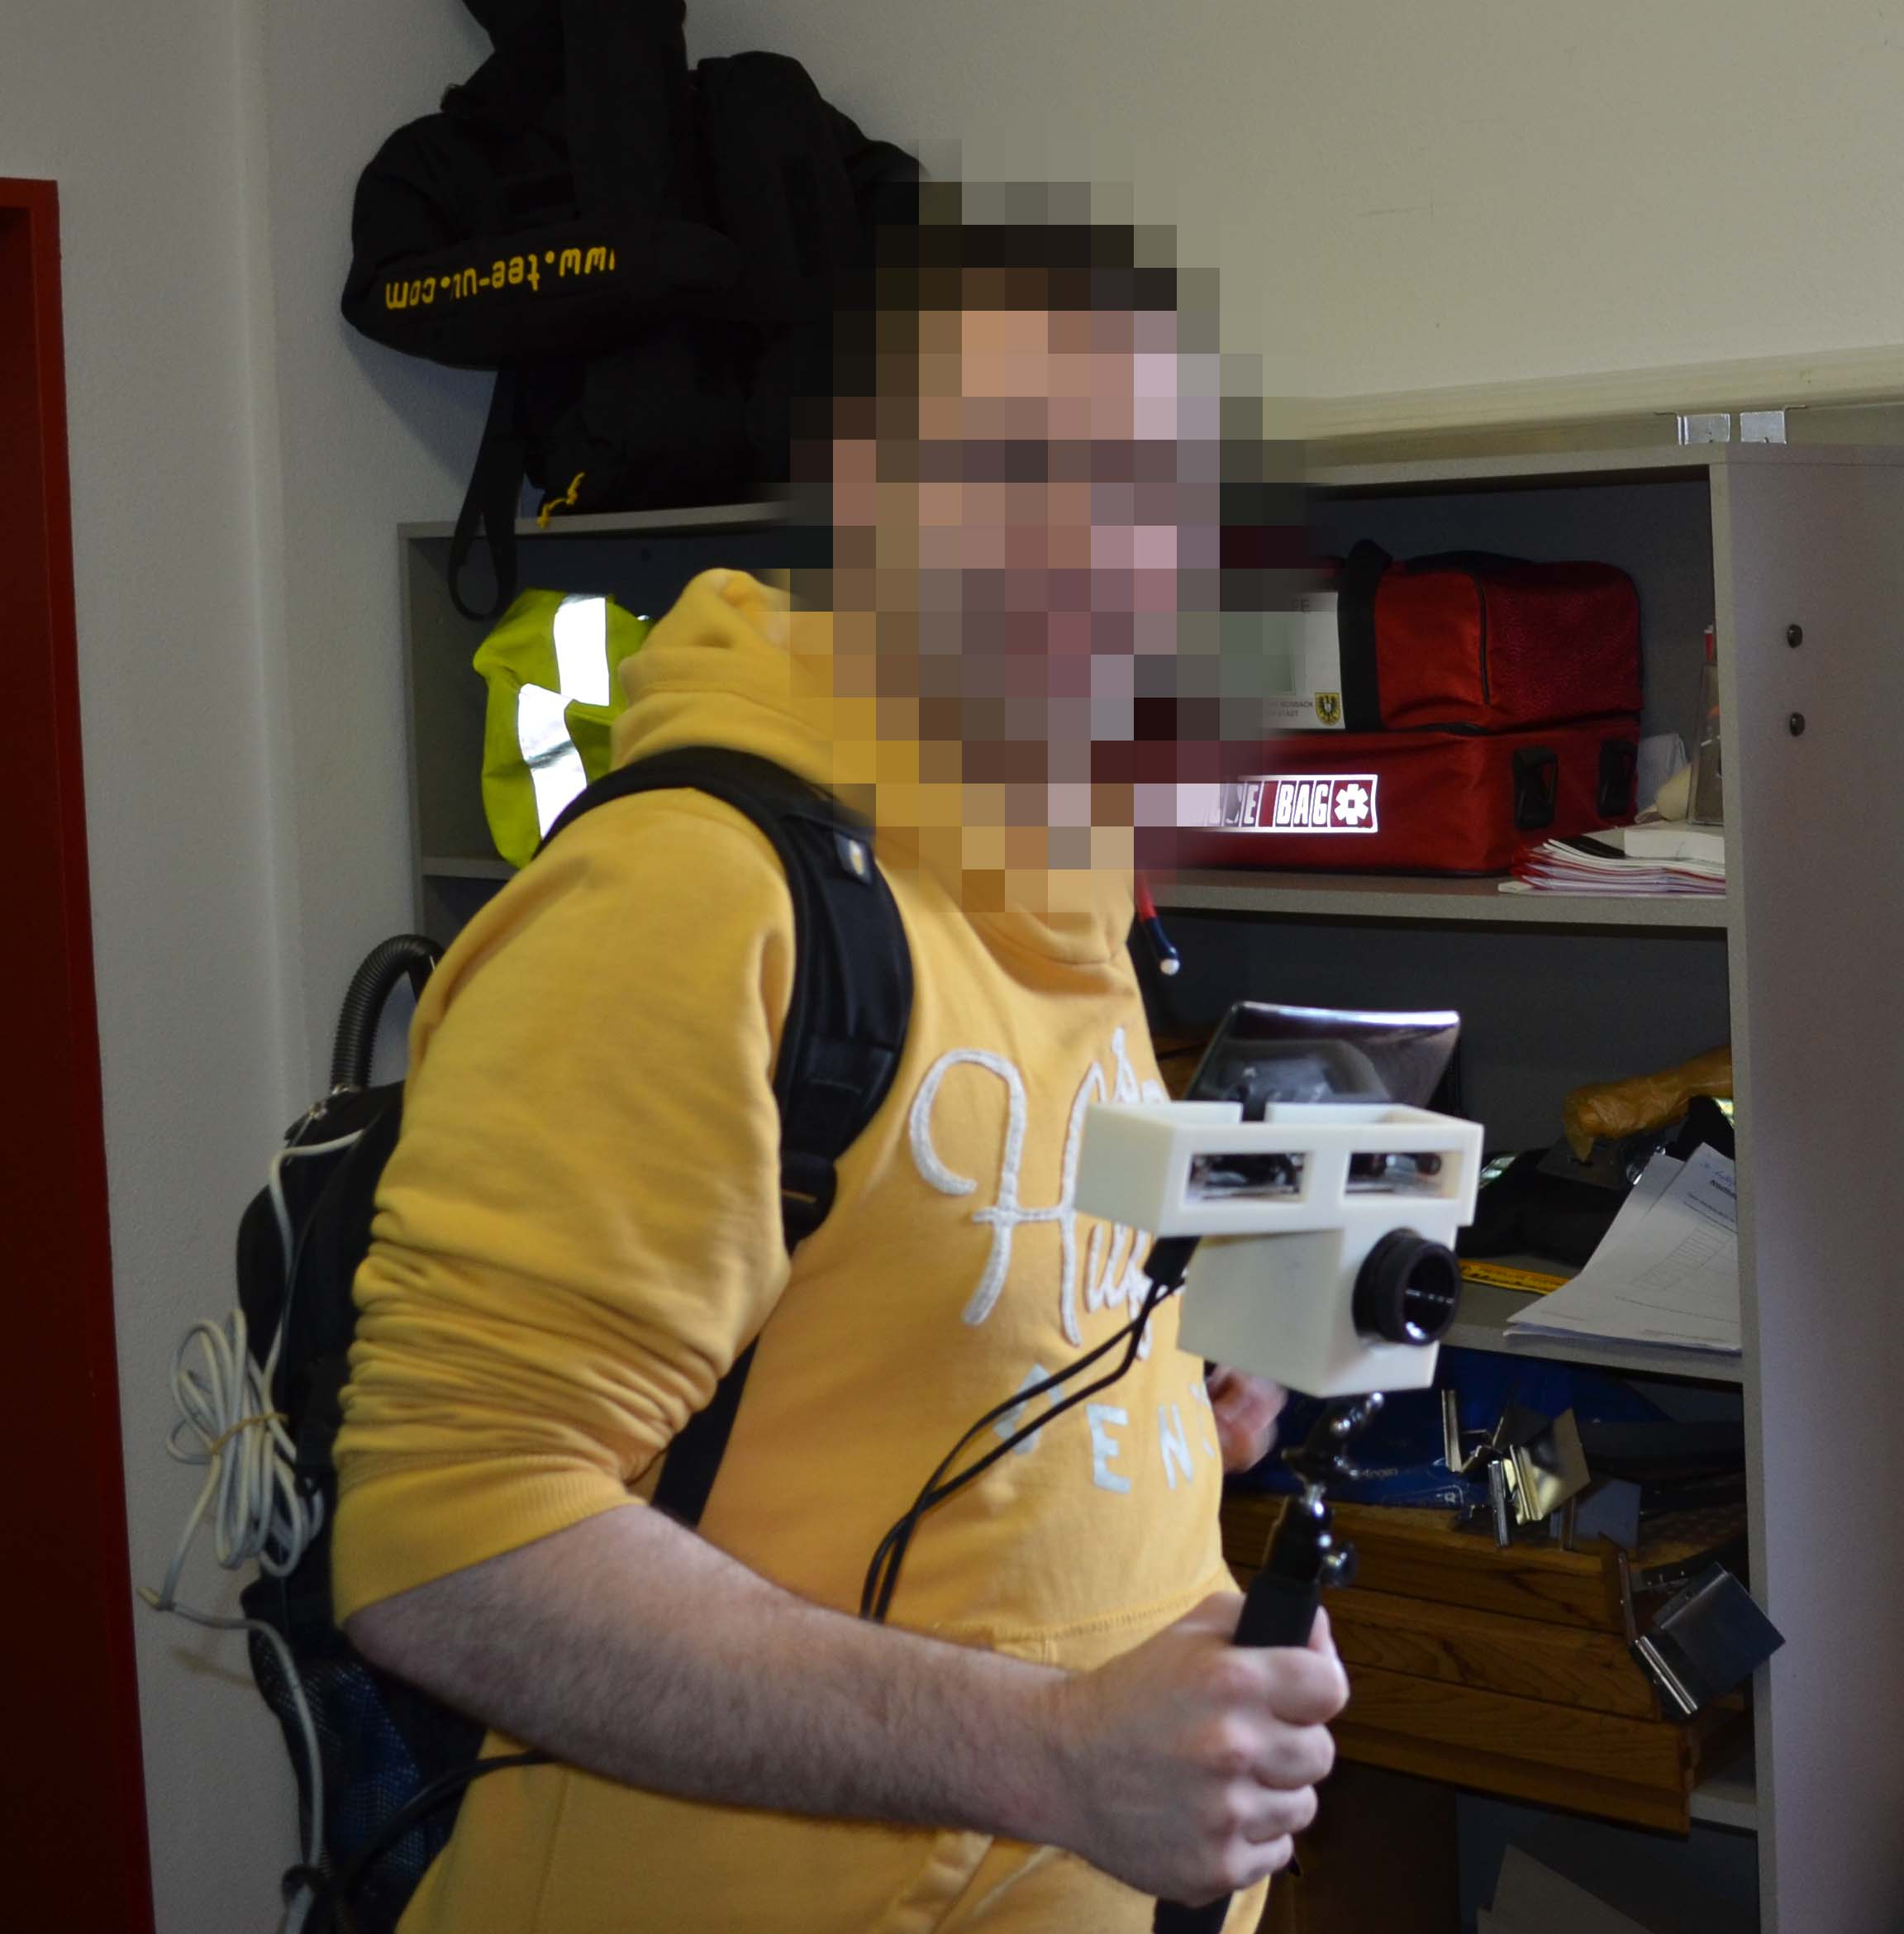
\includegraphics[width=\textwidth]{Spezi/handheld.jpg}}{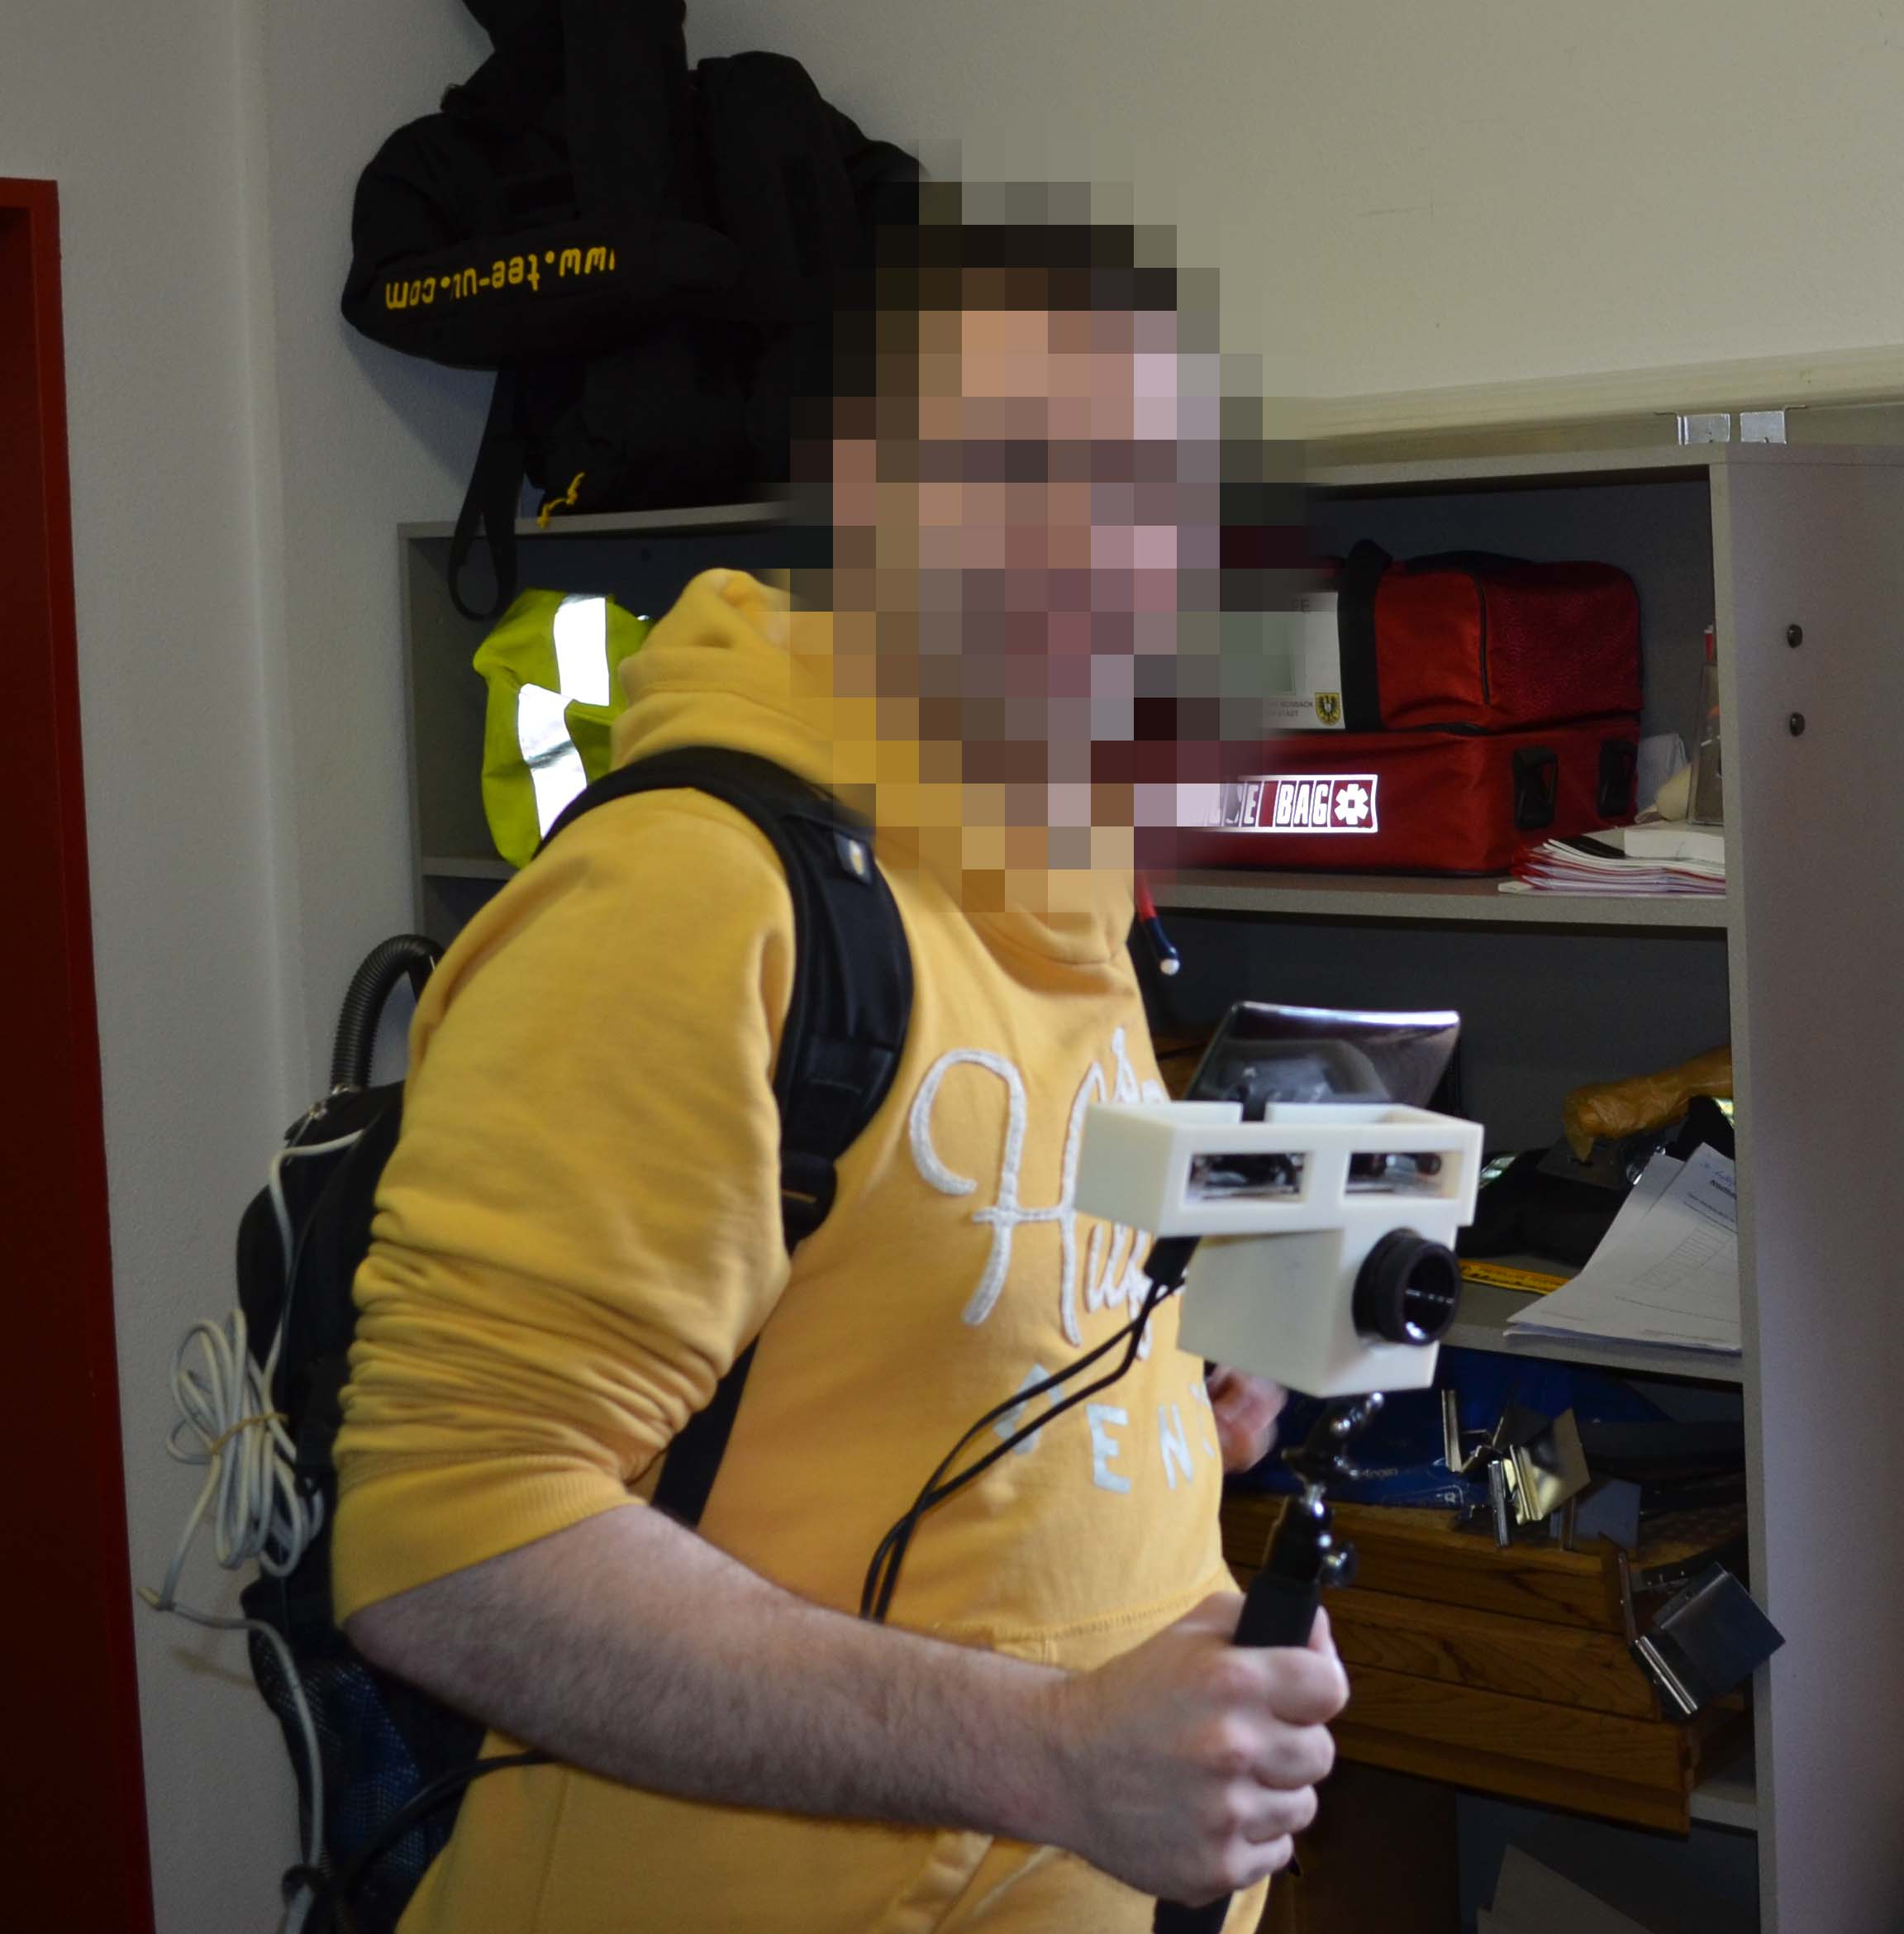
\includegraphics[width=\textwidth]{Spezi/handheld.png}}
		\caption{Handheld Prototyp}
		\label{fig:spezi_halterung_hand}
	\end{subfigure}
	~
	\begin{subfigure}[t]{0.45\textwidth}
		\centering
		\ifthenelse{\boolean{jpg}}{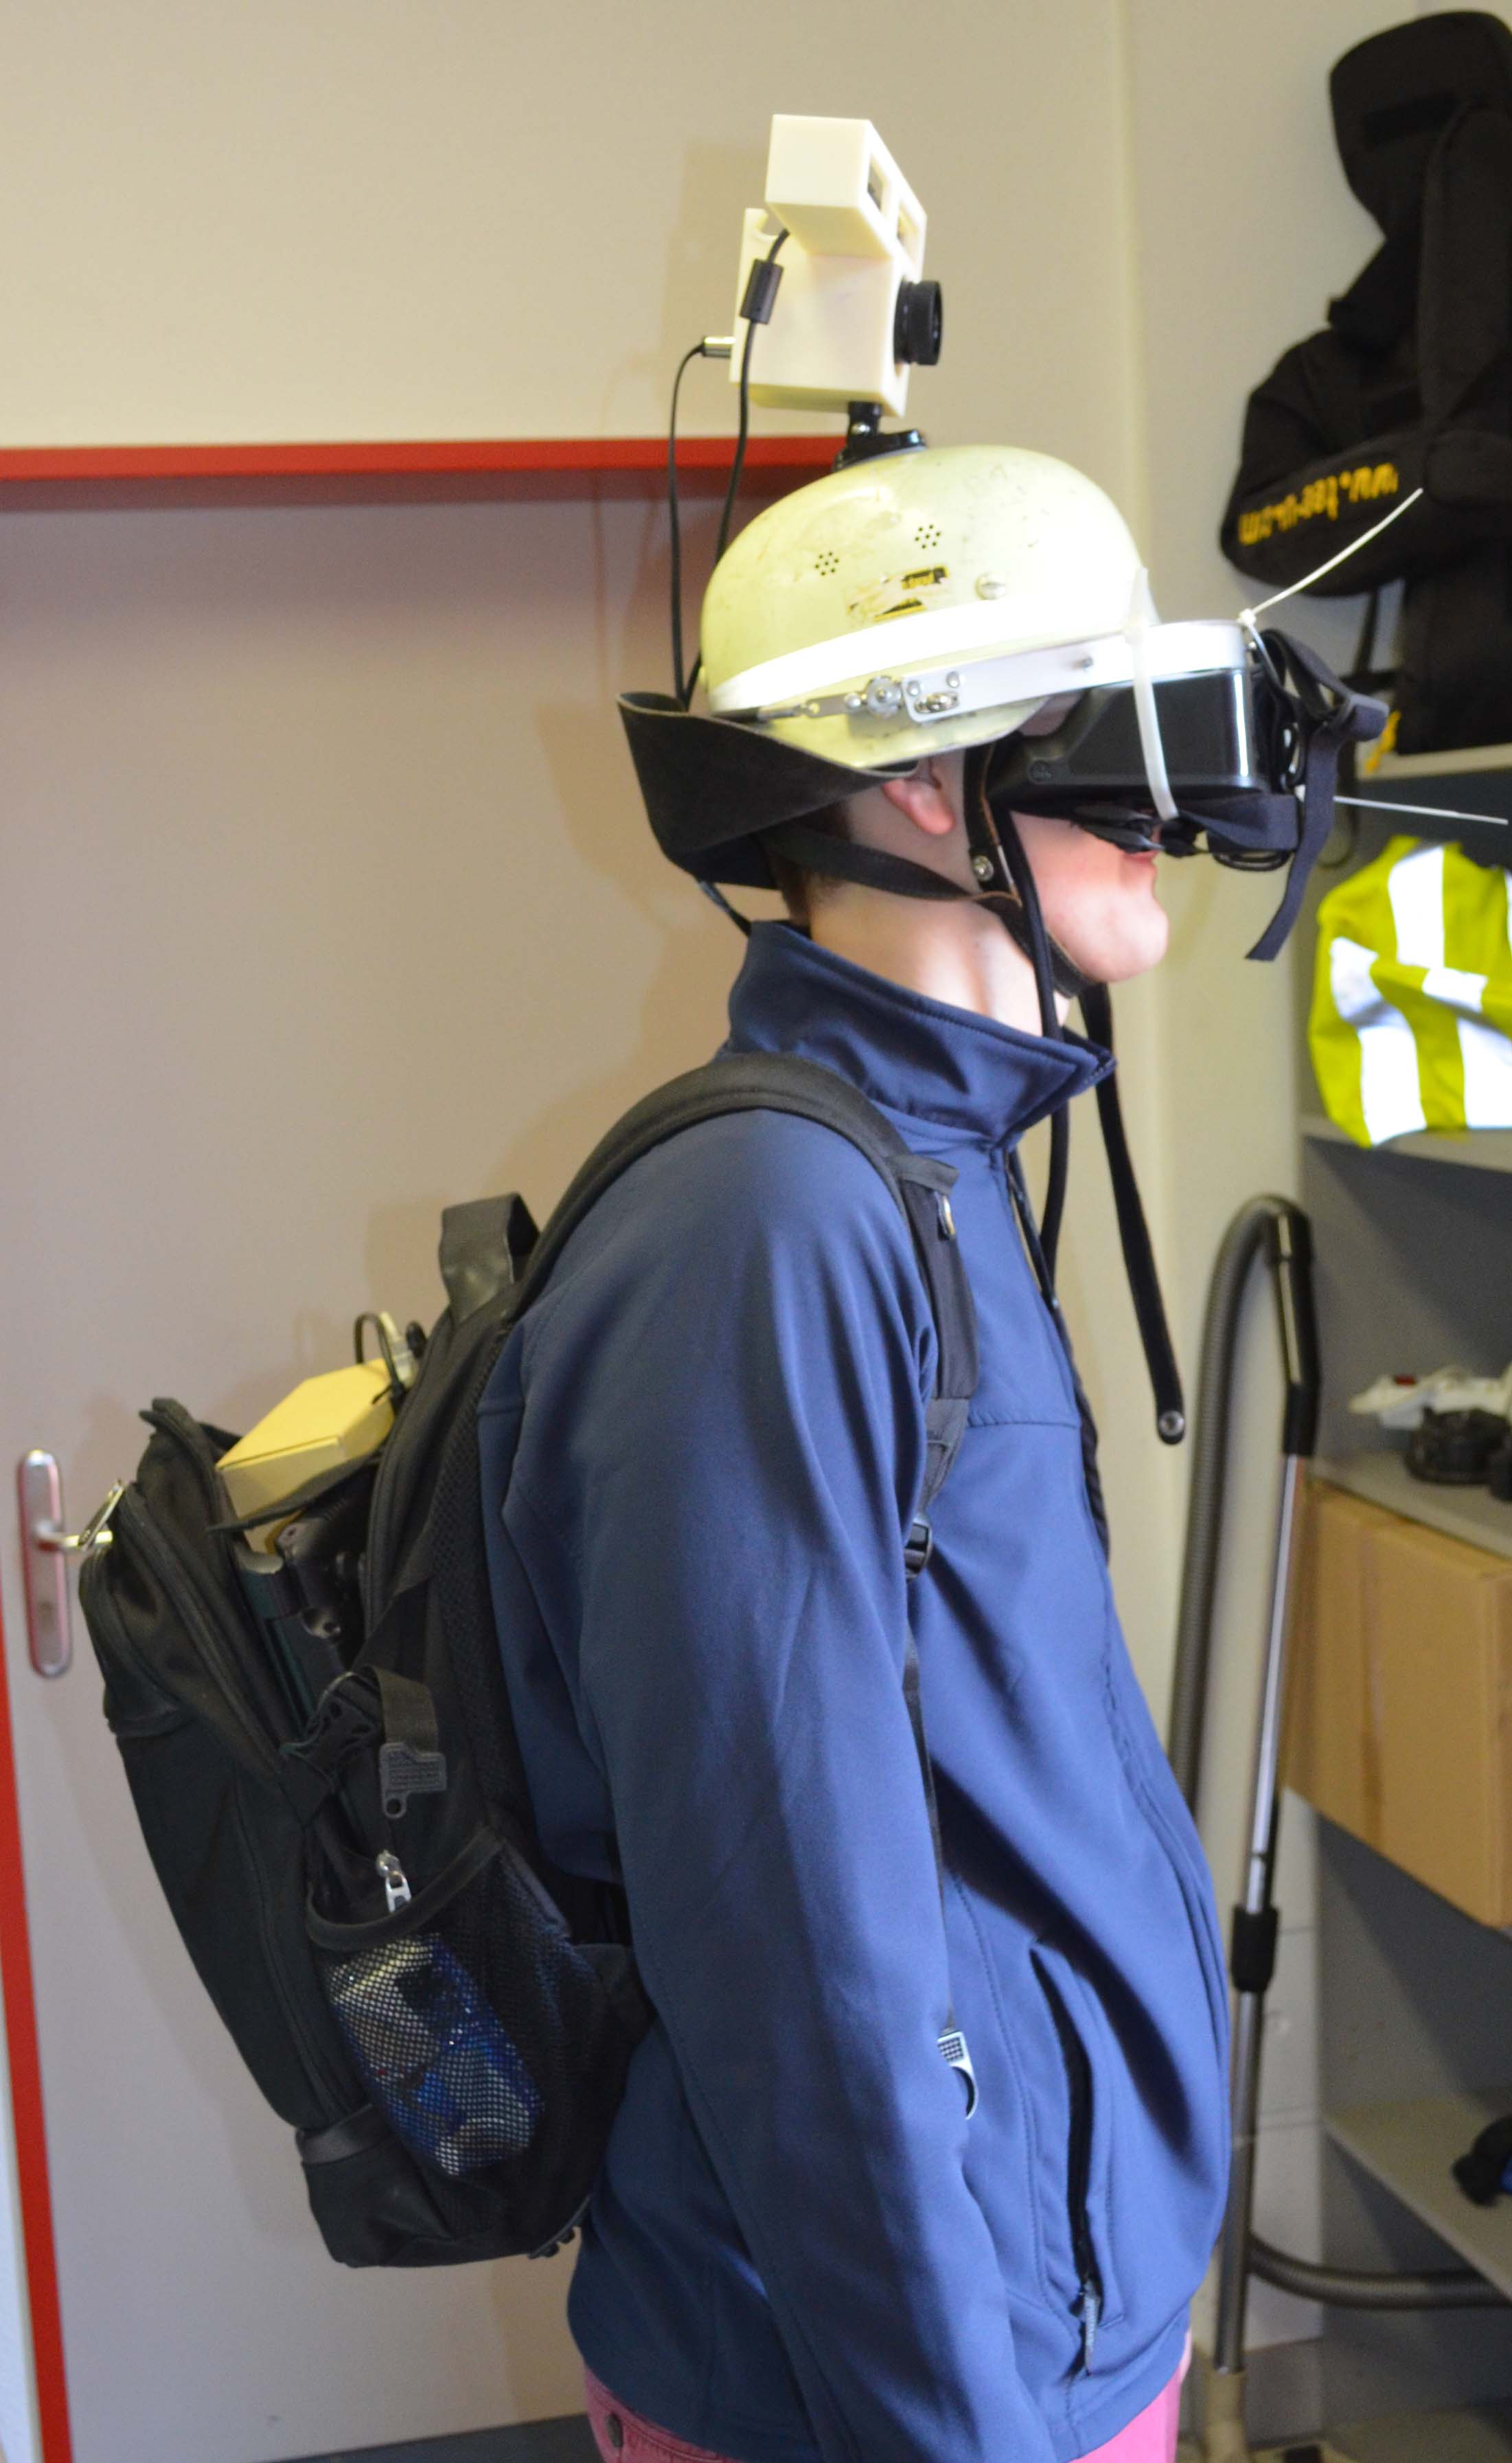
\includegraphics[scale=0.25]{Spezi/hmd.jpg}}{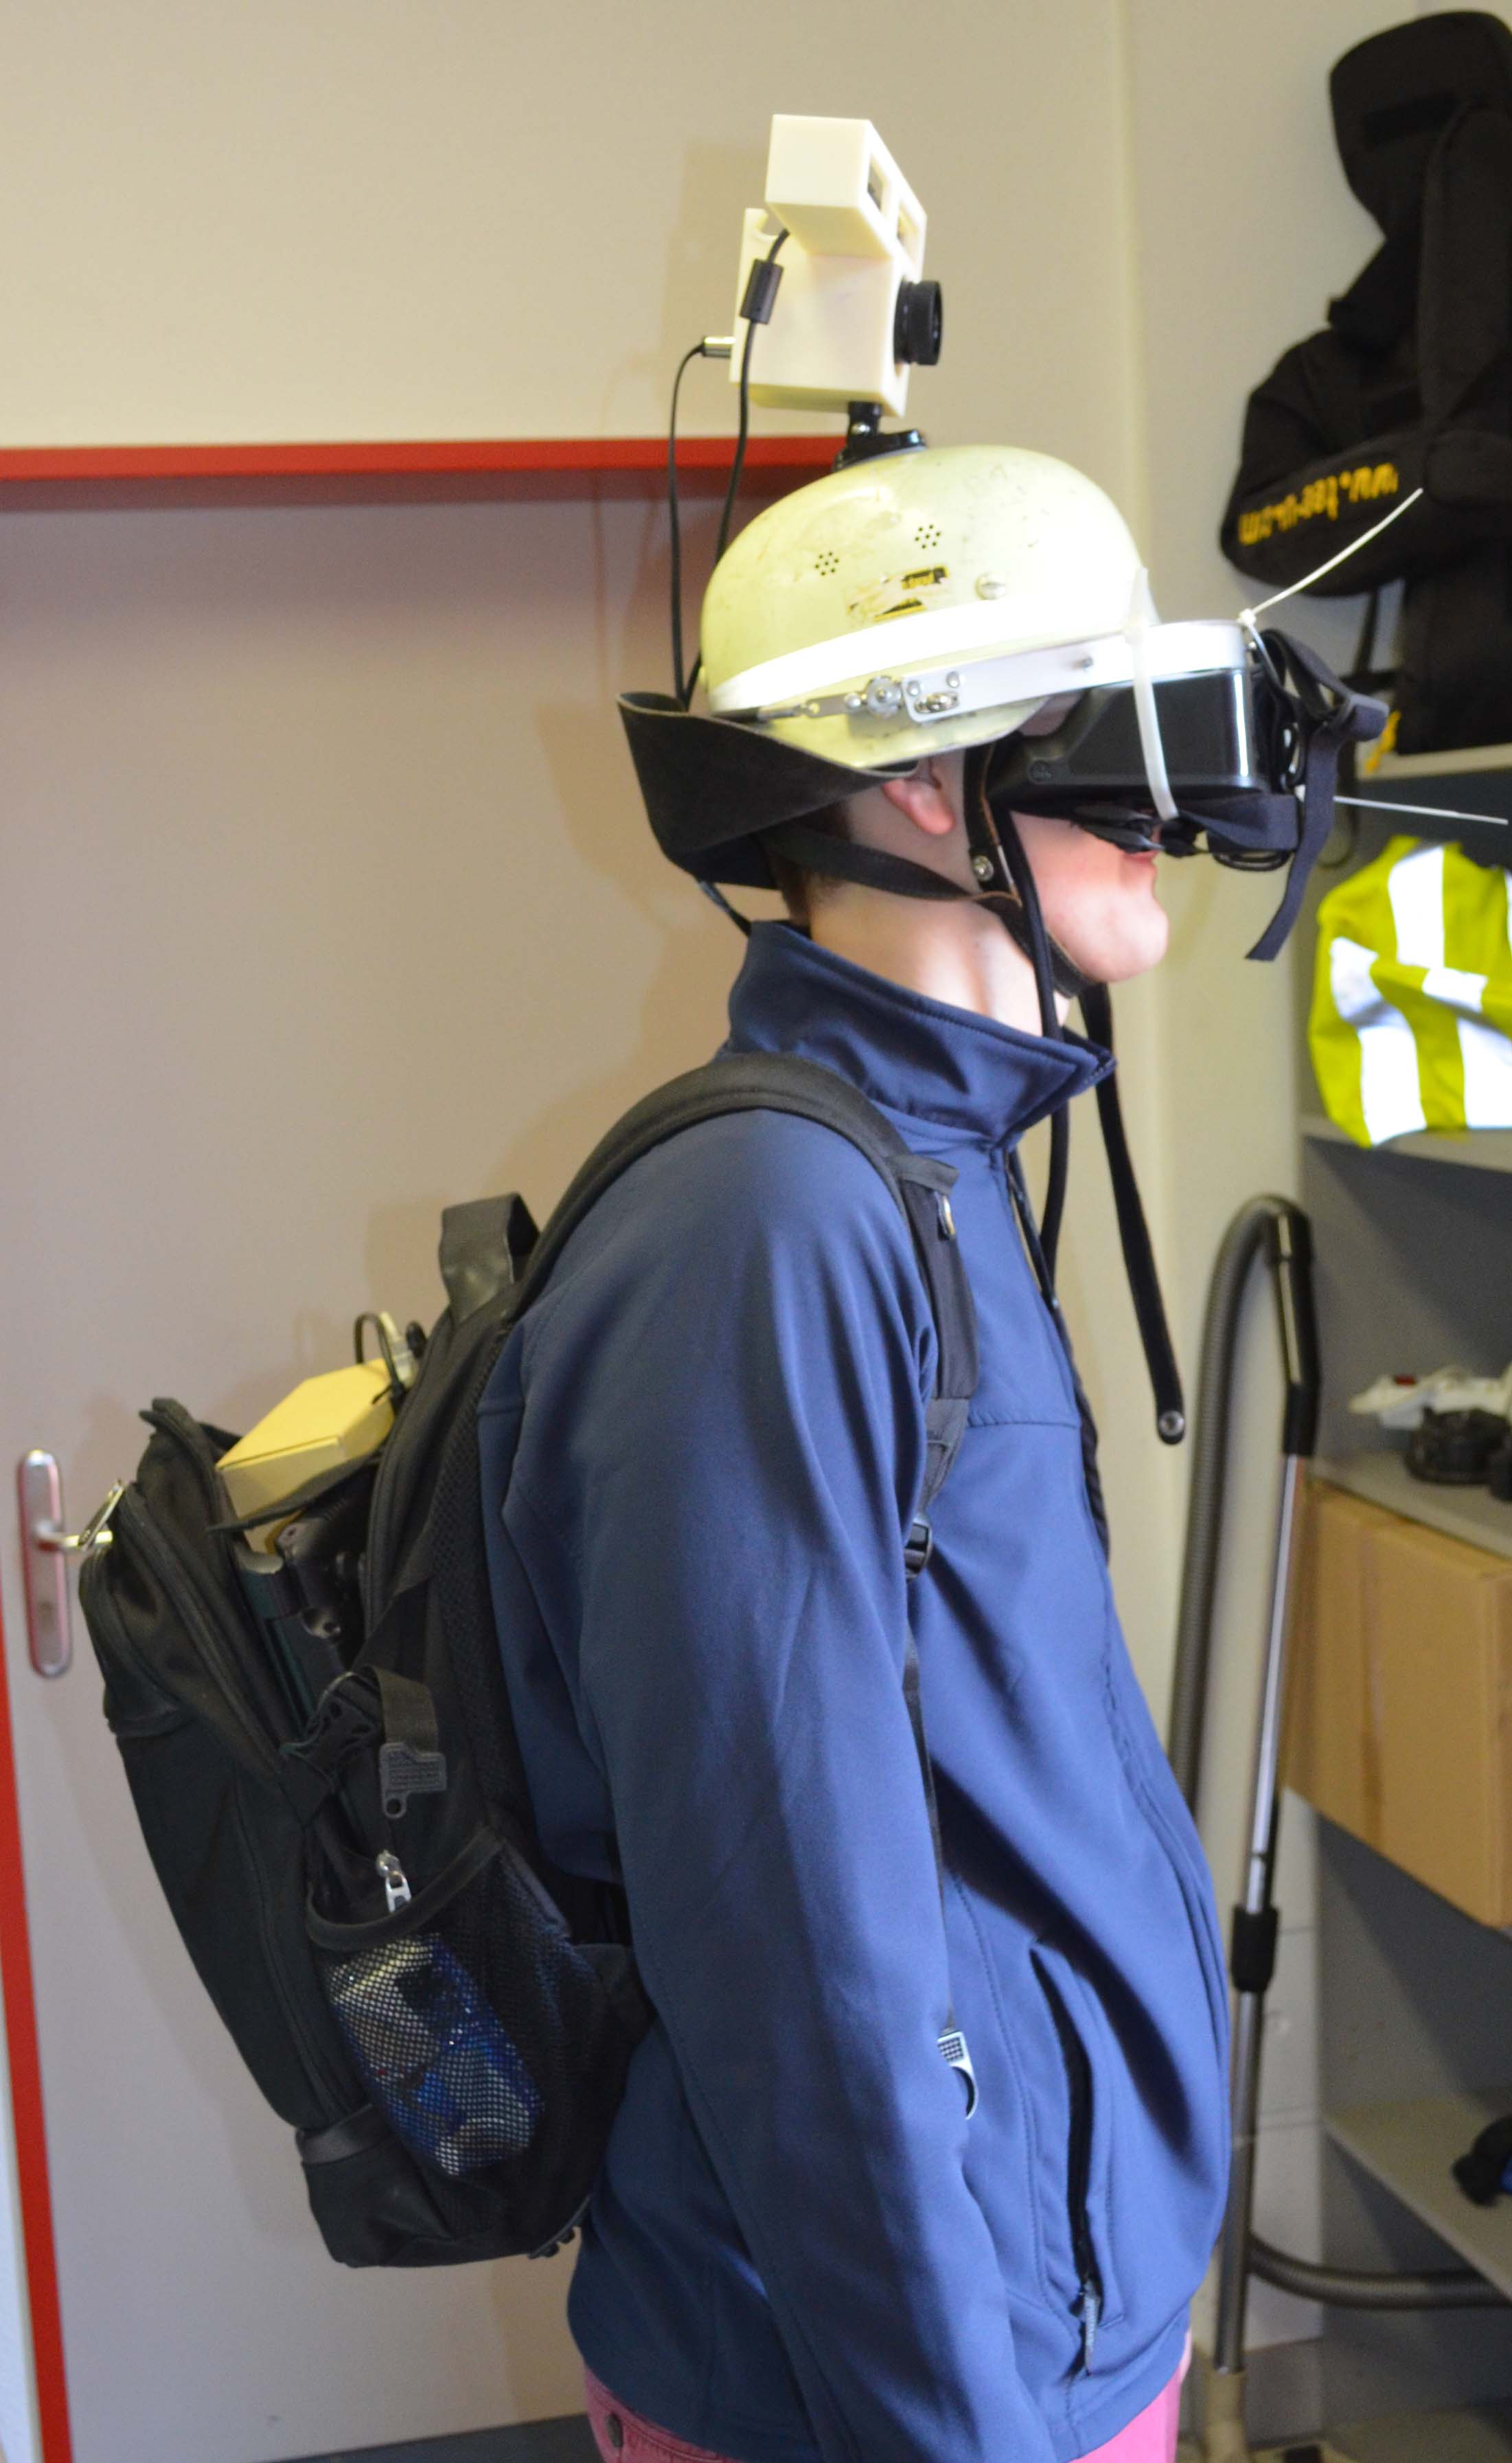
\includegraphics[scale=0.25]{Spezi/hmd.png}}
		\caption{Prototyp in Kombination mit einem Head Mounted Display}
		\label{fig:spezi_halterung_hmd}
	\end{subfigure}
	\caption{Halterungsaufbau}
	\label{fig:spezi_halterung}
\end{figure}

Die Wärmebildkamera und der \hyperlink{tab:tiefe}{Tiefenbild}sensor werden in einer gemeinsamen Halterung montiert.
Diese Halterung verfügt über ein Gewinde, welches eine Montage auf einem Standard GoPro-Handstativ ermöglicht.
Der Benutzer trägt die Halterung, über diesen Stick, per Hand.
Zusätzlich existiert die Möglichkeit, die Halterung an einem Feuerwehrhelm zu befestigen.

Die Programmsteuerung erfolgt über eine Maus oder ein mausähnliches Gerät, welches \ggf an der Halterung montiert ist.
Dabei werden lediglich die Maustasten zum Steuern benötigt.

Es sind zwei Ausgabemöglichkeiten vorgesehen, welche sich in ihrer Funktionalität nicht unterscheiden:
Erstere sieht so aus, dass der Benutzer eine Augmented Reality Brille (\meta) auf hat, welche am Laptop angeschlossen ist.
Hierbei kann der Benutzer über die AR Brille die verschiedenen Ausgabemethoden, wie Wärmebild, \hyperlink{tab:tiefe}{Tiefenbild} und beide fusioniert, direkt vor seinem Auge sehen.
Die zweite Variante funktioniert ähnlich wie die Erste.
Hierbei trägt der Benutzer ein mobiles Ausgabegerät (in unserem Fall ein Smartphone), welches \ggf sichtbar am Rücken der Halterung angebracht ist.
Das Ausgabegerät muss dafür im selben WLAN-Netz wie der Laptop sein.

Die GUI-Skizzen aus \cref{fig:spezi_mockup} geben einen Ausblick auf die anzustrebenden Ausgabemöglichkeiten:
\begin{figure}[t]
	\centering
	\begin{subfigure}[t]{0.45\textwidth}
		\centering
		\ifthenelse{\boolean{jpg}}{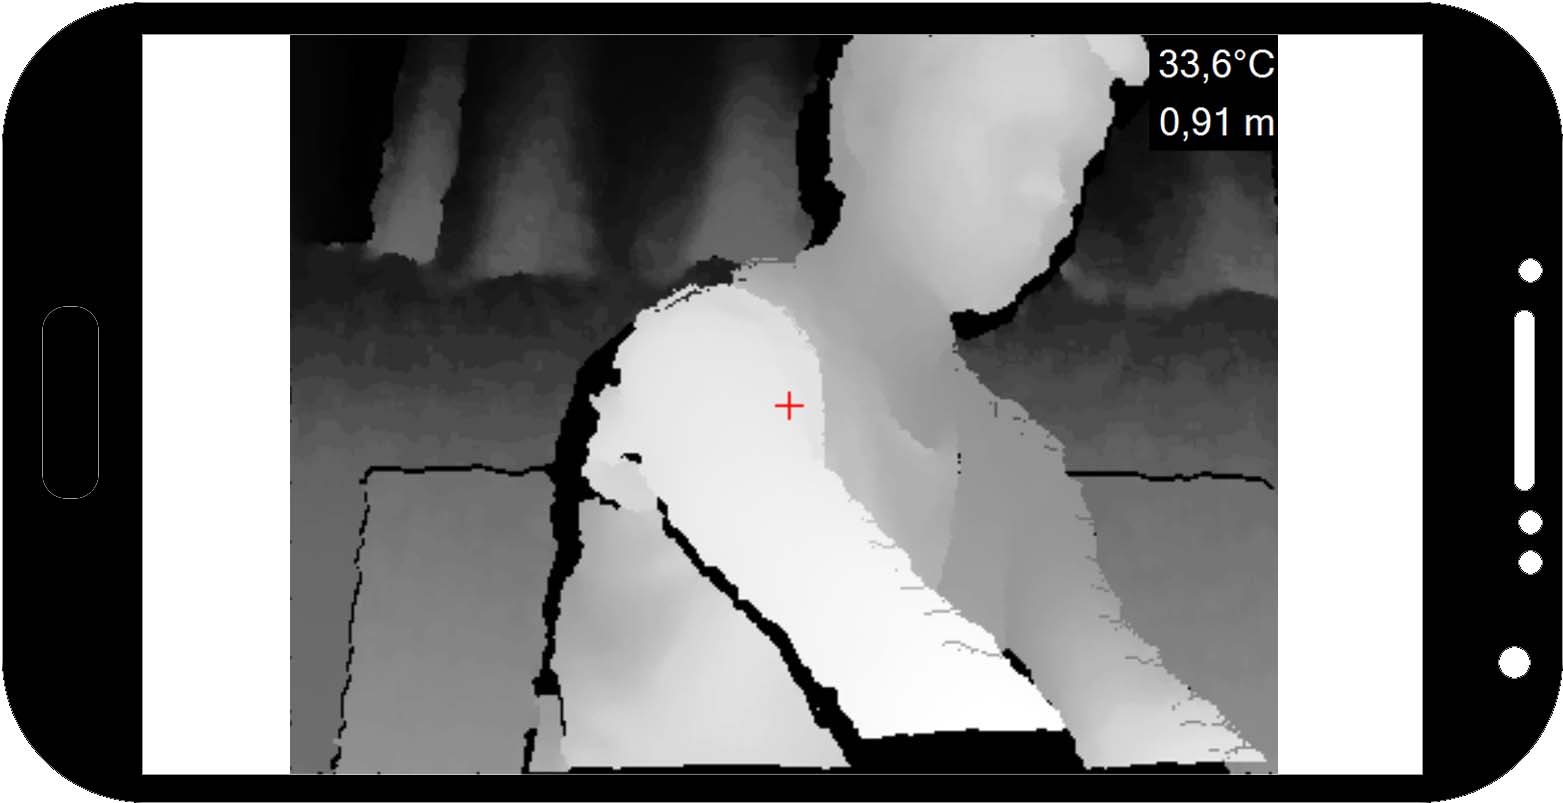
\includegraphics[width=\textwidth]{Spezi/depth_phone_mockup.jpg}}{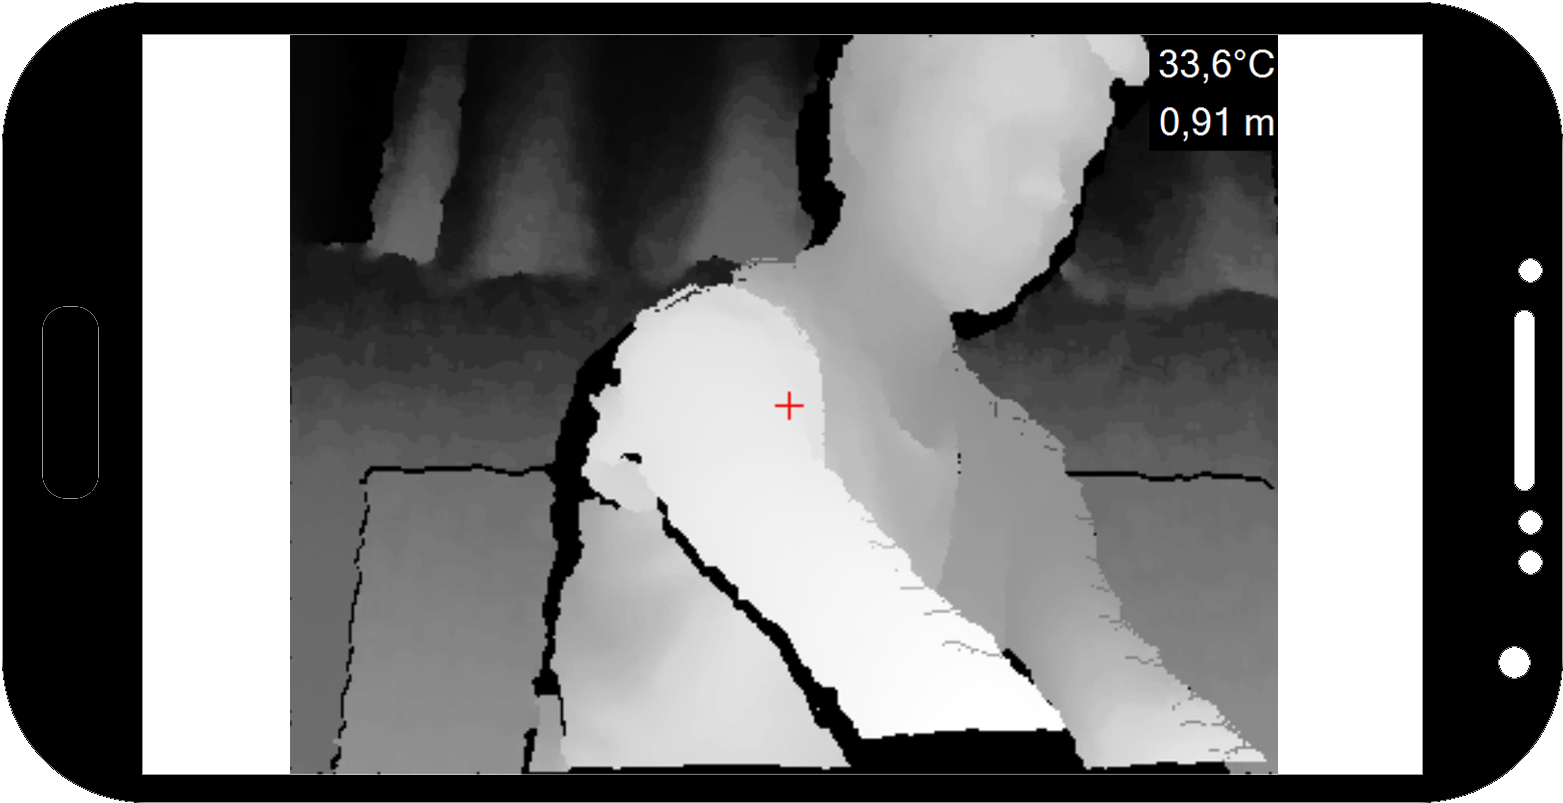
\includegraphics[width=\textwidth]{Spezi/depth_phone_mockup.png}}
		\caption{\hyperlink{tab:tiefe}{Tiefenbild}ausgabe auf mobilen Anzeigegerät}
		\label{fig:spezi_deepth_mockup}
	\end{subfigure}
	~
	\begin{subfigure}[t]{0.45\textwidth}
		\centering
		\ifthenelse{\boolean{jpg}}{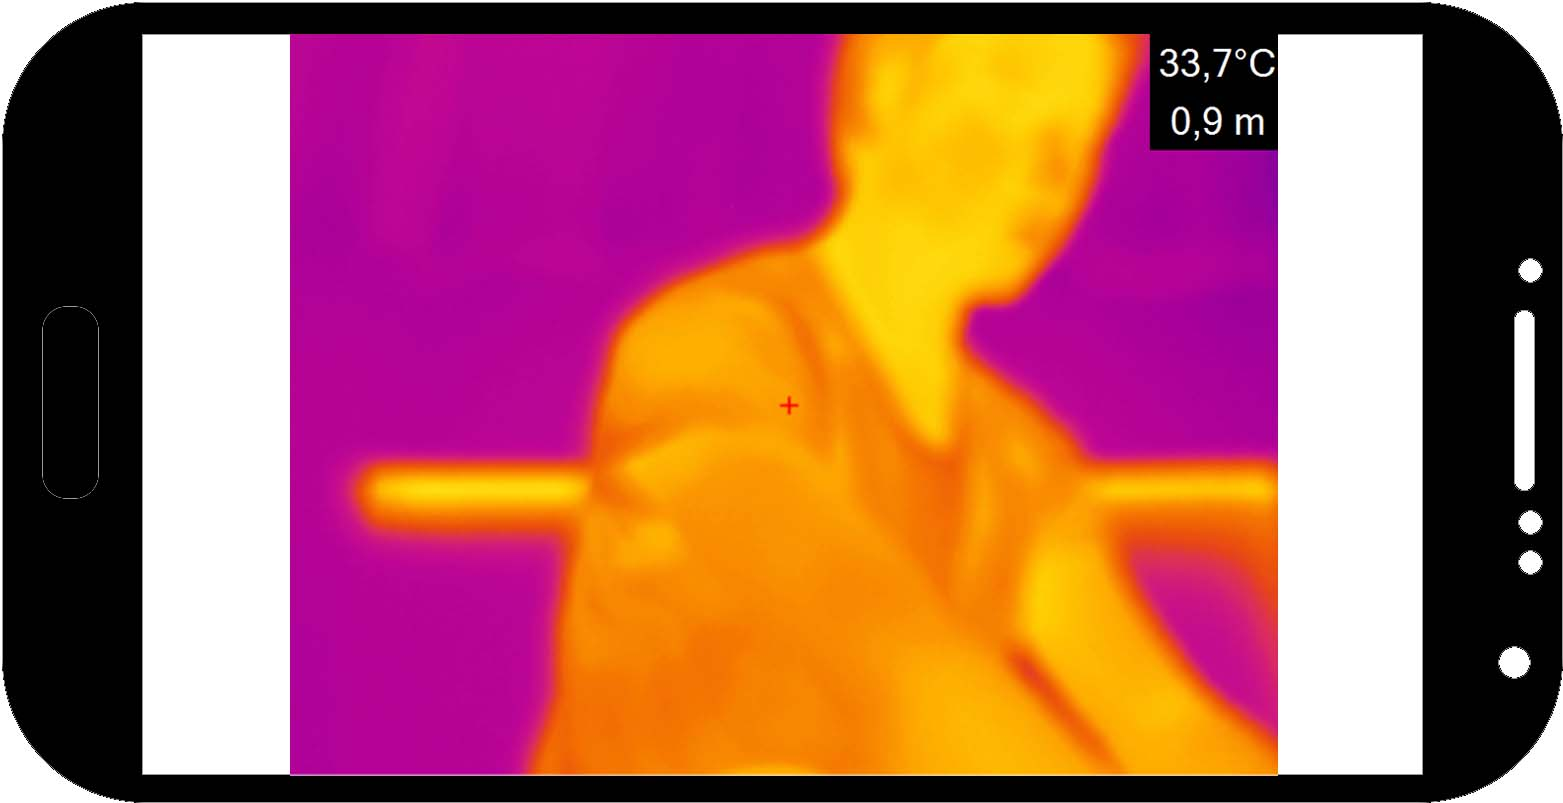
\includegraphics[width=\textwidth]{Spezi/heat_phone_mockup.jpg}}{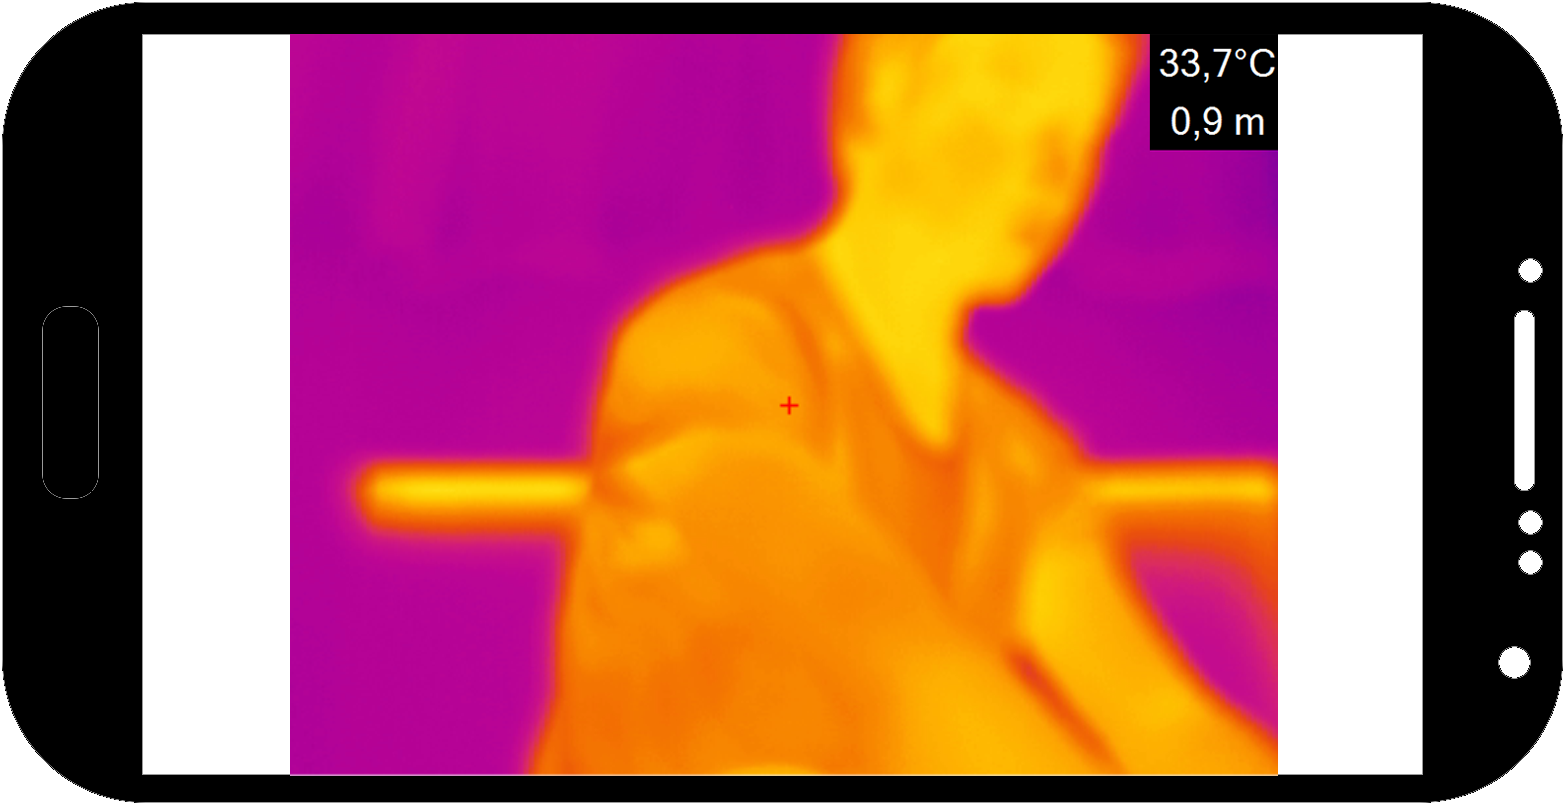
\includegraphics[width=\textwidth]{Spezi/heat_phone_mockup.png}}
		\caption{Wärmebildausgabe auf mobilen Anzeigegerät}
		\label{fig:spezi_heat_mockup}
	\end{subfigure}
	~
	\begin{subfigure}[t]{0.45\textwidth}
		\centering
		\ifthenelse{\boolean{jpg}}{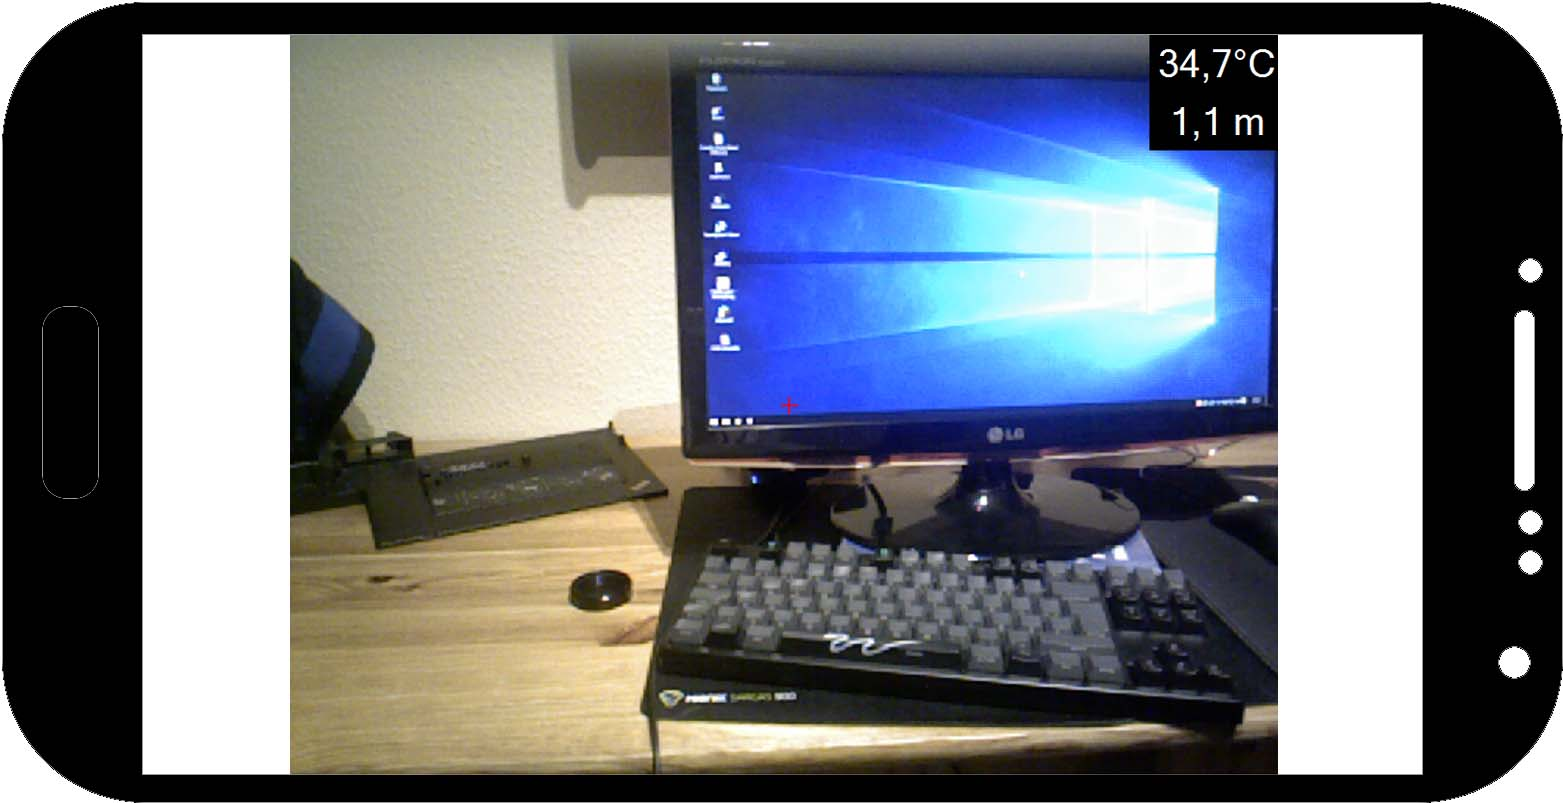
\includegraphics[width=\textwidth]{Spezi/rgb_phone_mockup.jpg}}{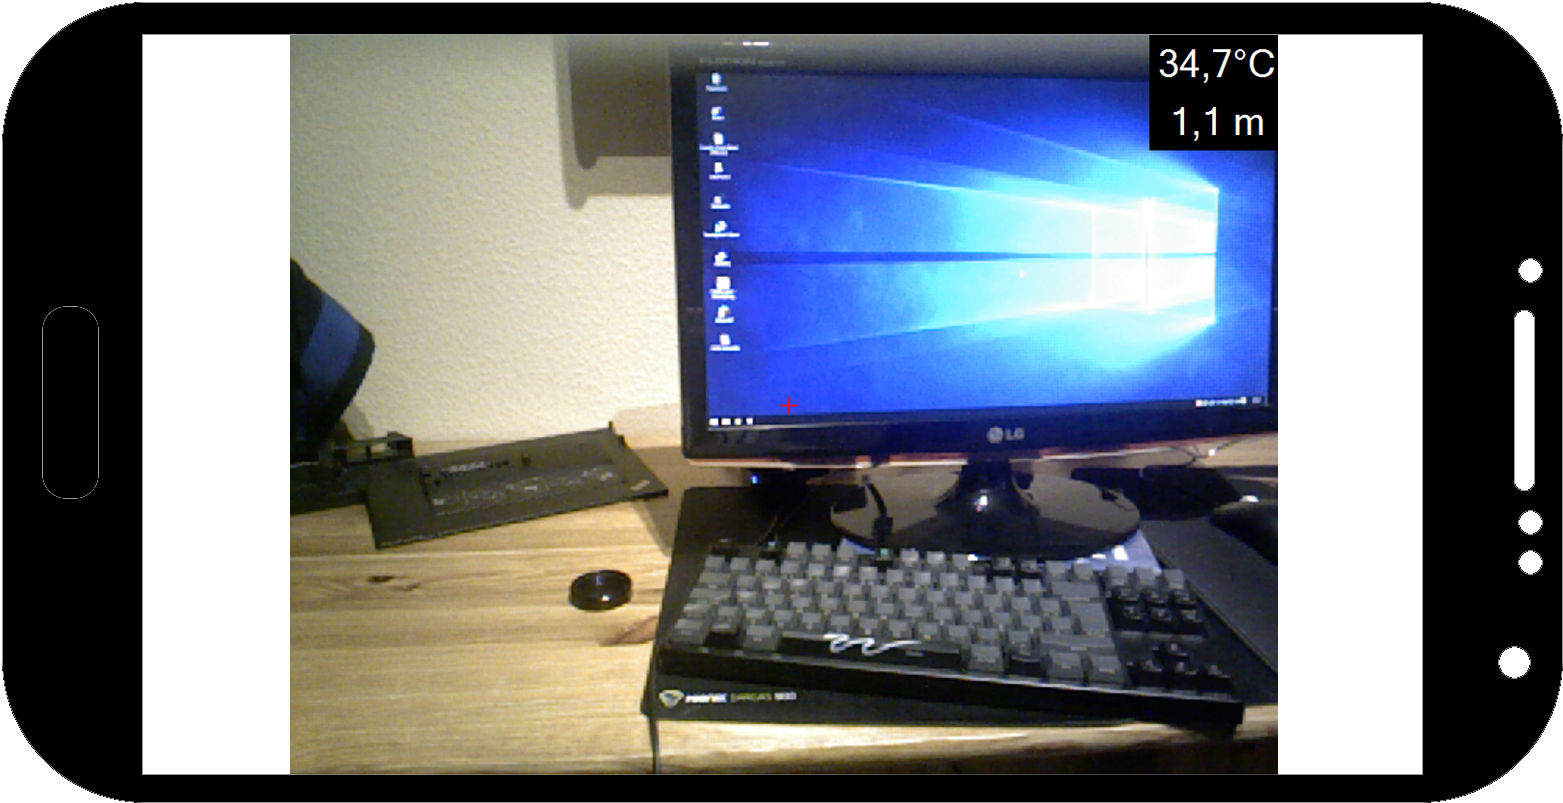
\includegraphics[width=\textwidth]{Spezi/rgb_phone_mockup.png}}
		\caption{RBG-Bildausgabe auf mobilen Anzeigegerät}
		\label{fig:spezi_rgb_mockup}
	\end{subfigure}
	~
	\begin{subfigure}[t]{0.45\textwidth}
		\centering
		\ifthenelse{\boolean{jpg}}{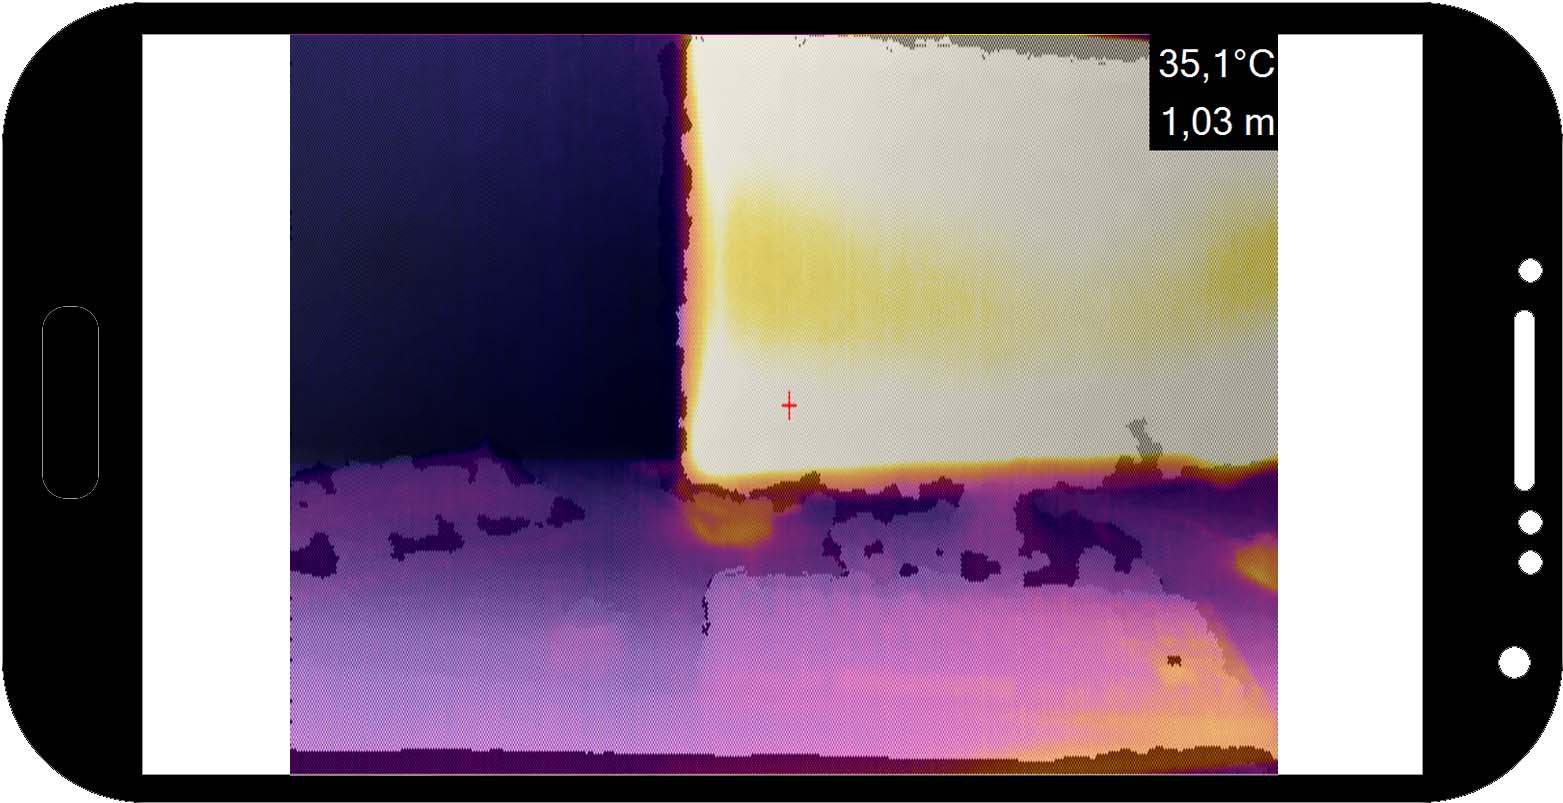
\includegraphics[width=\textwidth]{Spezi/fus_phone_mockup.jpg}}{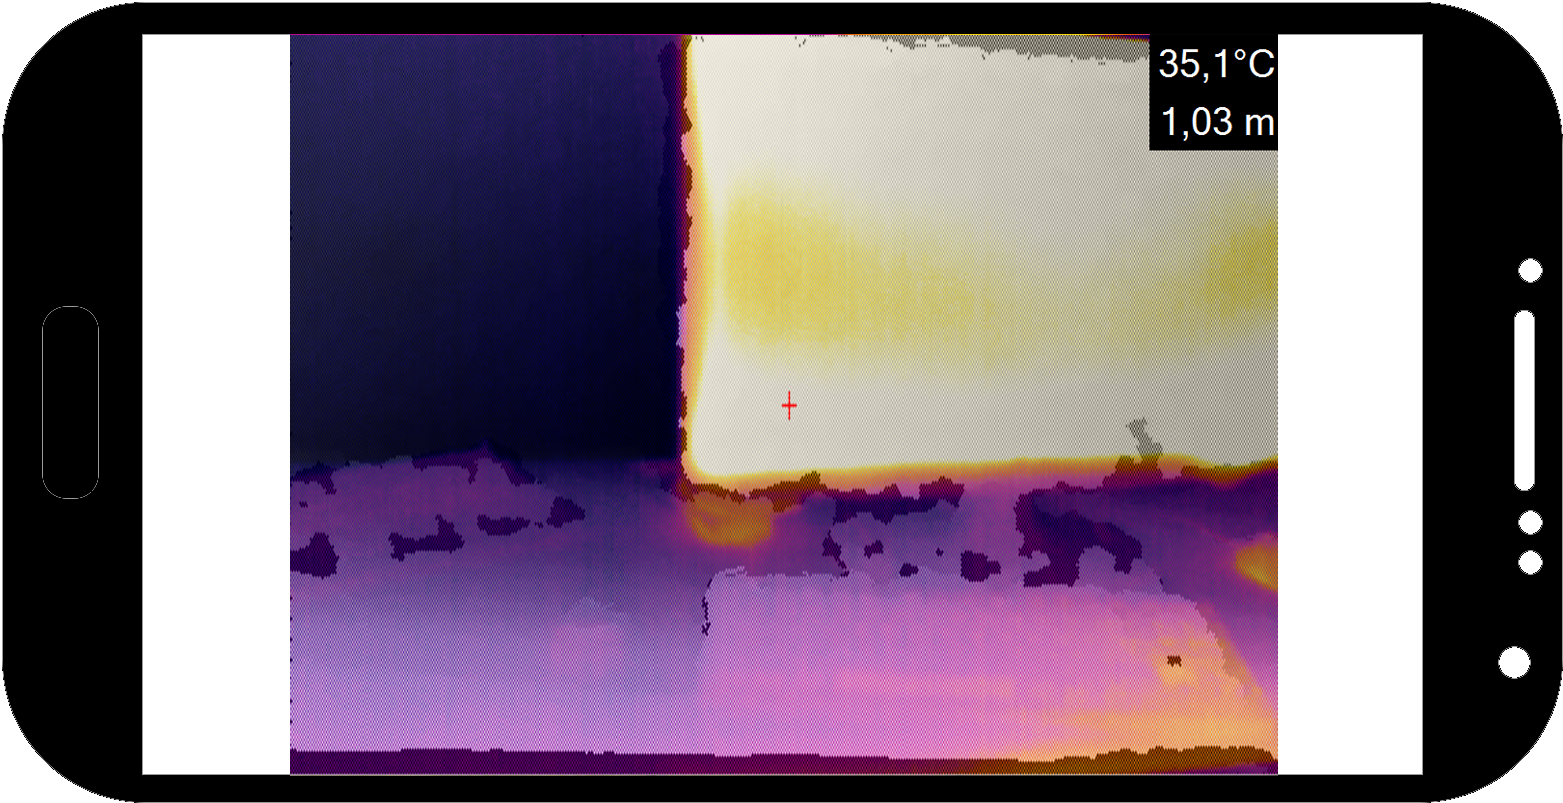
\includegraphics[width=\textwidth]{Spezi/fus_phone_mockup.png}}
		\caption{Erstellte Fusionsausgabe auf mobilen Anzeigegerät}
		\label{fig:spezi_fus_mockup}
	\end{subfigure}
	\caption{Mock-Ups der Ausgabe auf einem mobilen Anzeigegerät}
	\label{fig:spezi_mockup}
\end{figure}

\section{Anwendungsfälle}
\label{chap:spezi_usecases}

\subsection{Anwendungsfalldiagramm}
\begin{figure}[H]
	\centering
	\ifthenelse{\boolean{jpg}}{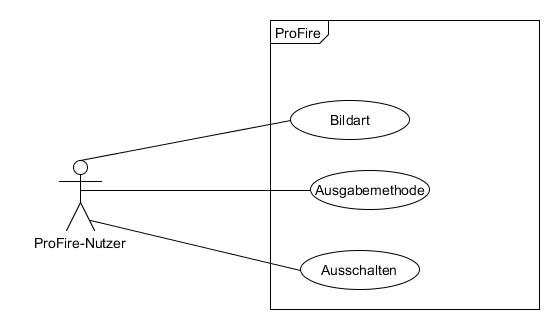
\includegraphics[width=0.8\textwidth]{Spezi/profire.jpg}}{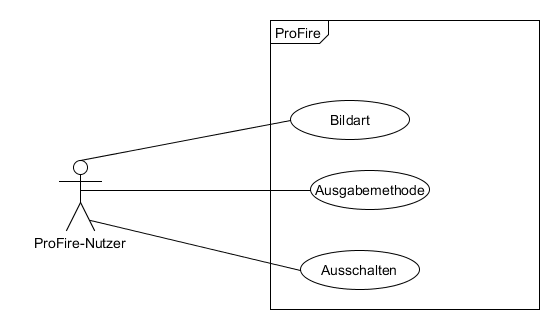
\includegraphics[width=0.8\textwidth]{Spezi/profire.png}}
	\caption{Zeigt die Funktionen von \profire}
	\label{fig:spezi_profire}
\end{figure}
\begin{figure}[H]
	\centering
	\ifthenelse{\boolean{jpg}}{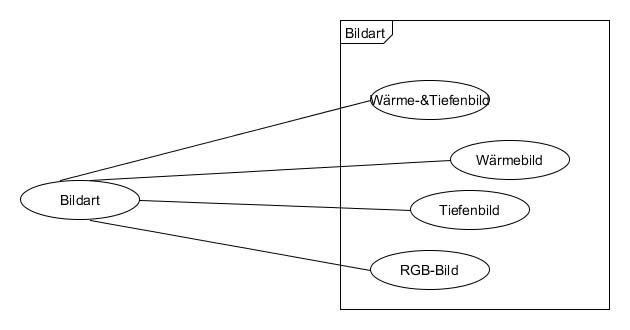
\includegraphics[width=0.8\textwidth]{Spezi/pic.jpg}}{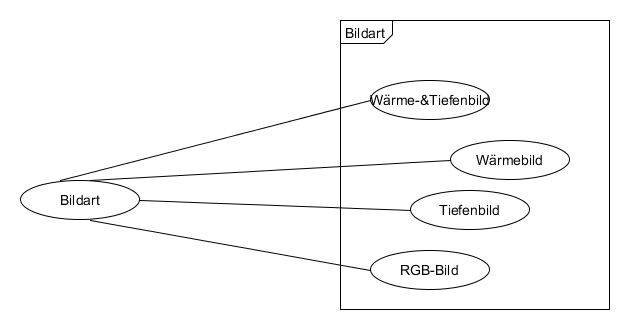
\includegraphics[width=0.8\textwidth]{Spezi/pic.png}}
	\caption{Zeigt die genauen Funktionen von Bildart}
	\label{fig:spezi_pic}
\end{figure}
\begin{figure}[H]
	\centering
	\ifthenelse{\boolean{jpg}}{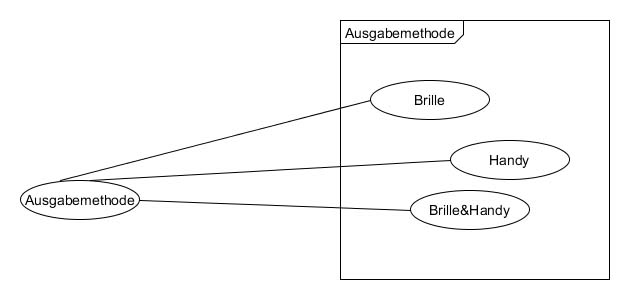
\includegraphics[width=0.8\textwidth]{Spezi/output.jpg}}{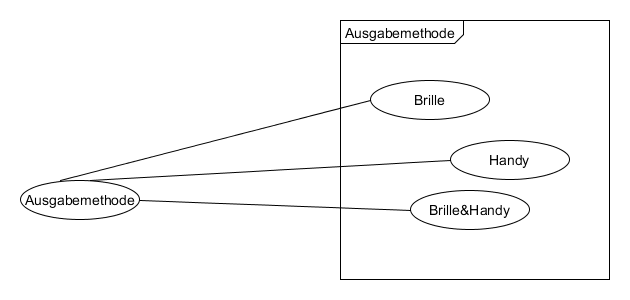
\includegraphics[width=0.8\textwidth]{Spezi/output.png}}
	\caption{Zeigt die genauen Funktionen von Ausgabemethode}
	\label{fig:spezi_output}
\end{figure}

\subsection{Beschreibung der Anwendungsfälle}
In den folgenden Anwendungsfälle wird davon ausgegangen, dass sowohl die Brille aus auch das mobile Anzeigegerät zur Bildausgabe genutzt wird.

\subsubsection{Das Tiefebild anzeigen}
\begin{center}
	\begin{longtable}{| p{3cm} | p{12cm} |}
		\hline
		\goal & Der Nutzer kann das \hyperlink{tab:tiefe}{Tiefenbild} sehen. \\ \hline
		
		\precondition & \begin{itemize}
			\item Die \hyperlink{tab:anwendung}{Software} wurde ordnungsgemäß gestartet.
			\item Die \hyperlink{tab:anwendung}{Software} zeigt nicht das \hyperlink{tab:tiefe}{Tiefenbild} an.
		\end{itemize} \\ \hline
		
		\postcondition & \begin{itemize}
			\item Das \hyperlink{tab:tiefe}{Tiefenbild} wird auf der Brille und auf dem mobilen Anzeigegerät angezeigt.
		\end{itemize} \\ \hline
		
		\postexception & --- \\ \hline
		
		\flow & \begin{enumerate}
			\item Der Nutzer betätigt den Linksklick der Maus.
			\item Es werden für jeden Klick nacheinander die verschiedenen Bildmodi angezeigt.
			\item Der Nutzer betätigt den Linksklick der Maus bis das \hyperlink{tab:tiefe}{Tiefenbild} angezeigt wird.
			\item Das \hyperlink{tab:tiefe}{Tiefenbild} wird angezeigt.			
		\end{enumerate} \\ \hline
		
		\exception & --- \\ \hline
		
		\player & Der Nutzer \\
		\hline
	\end{longtable}
\end{center}

\subsubsection{Das Wärmebild anzeigen}
\begin{center}
	\begin{longtable}{| p{3cm} | p{12cm} |}
		\hline
		\goal & Der Nutzer kann das Wärmebild sehen. \\ \hline
		
		\precondition & \begin{itemize}
			\item Die \hyperlink{tab:anwendung}{Software} wurde ordnungsgemäß gestartet.
			\item Die \hyperlink{tab:anwendung}{Software} zeigt nicht das Wärmebild an.
		\end{itemize} \\ \hline
		
		\postcondition & \begin{itemize}
			\item Das Wärmebild wird auf der Brille und auf dem mobilen Anzeigegerät angezeigt.
		\end{itemize} \\ \hline
		
		\postexception & --- \\ \hline
		
		\flow & \begin{enumerate}
			\item Der Nutzer betätigt den Linksklick der Maus.
			\item Es werden für jeden Klick nacheinander die verschiedenen Bildmodi angezeigt.
			\item Der Nutzer betätigt den Linksklick der Maus bis das Wärmebild angezeigt wird.
			\item Das Wärmebild wird angezeigt.			
		\end{enumerate} \\ \hline
		
		\exception & --- \\ \hline
		
		\player & Der Nutzer \\
		\hline
	\end{longtable}
\end{center}

\subsubsection{Das verbesserte Wärmebild anzeigen}
\begin{center}
	\begin{longtable}{| p{3cm} | p{12cm} |}
		\hline
		\goal & Der Nutzer kann das verbesserte Wärmebild sehen. \\ \hline
		
		\precondition & \begin{itemize}
			\item Die \hyperlink{tab:anwendung}{Software} wurde ordnungsgemäß gestartet.
			\item Die \hyperlink{tab:anwendung}{Software} zeigt nicht das verbesserte Wärmebild an.
		\end{itemize} \\ \hline
		
		\postcondition & \begin{itemize}
			\item Das verbesserte Wärmebild wird auf der Brille und auf dem mobilen Anzeigegerät angezeigt.
		\end{itemize} \\ \hline
		
		\postexception & --- \\ \hline
		
		\flow & \begin{enumerate}
			\item Der Nutzer betätigt den Linksklick der Maus.
			\item Es werden für jeden Klick nacheinander die verschiedenen Bildmodi angezeigt.
			\item Der Nutzer betätigt den Linksklick der Maus bis das verbesserte Wärmebild angezeigt wird.
			\item Das verbesserte Wärmebild wird angezeigt.			
		\end{enumerate} \\ \hline
		
		\exception & --- \\ \hline
		
		\player & Der Nutzer \\
		\hline
	\end{longtable}
\end{center}

\subsubsection{Das RGB-Bild anzeigen}
\begin{center}
	\begin{longtable}{| p{3cm} | p{12cm} |}
		\hline
		\goal & Der Nutzer kann das RGB-Bild sehen. \\ \hline
		
		\precondition & \begin{itemize}
			\item Die \hyperlink{tab:anwendung}{Software} wurde ordnungsgemäß gestartet.
			\item Die \hyperlink{tab:anwendung}{Software} zeigt nicht das RGB-Bild an.
		\end{itemize} \\ \hline
		
		\postcondition & \begin{itemize}
			\item Das RGB-Bild wird auf der Brille und auf dem mobilen Anzeigegerät angezeigt.
		\end{itemize} \\ \hline
		
		\postexception & --- \\ \hline
		
		\flow & \begin{enumerate}
			\item Der Nutzer betätigt den Linksklick der Maus.
			\item Es werden für jeden Klick nacheinander die verschiedenen Bildmodi angezeigt.
			\item Der Nutzer betätigt den Linksklick der Maus bis das RGB-Bild angezeigt wird.
			\item Das RGB-Bild wird angezeigt.			
		\end{enumerate} \\ \hline
		
		\exception & --- \\ \hline
		
		\player & Der Nutzer \\
		\hline
	\end{longtable}
\end{center}

\subsubsection{Ausgabe auf der Brille deaktivieren}
\begin{center}
	\begin{longtable}{| p{3cm} | p{12cm} |}
		\hline
		\goal & Es findet keine Ausgabe auf der Brille statt. \\ \hline
		
		\precondition & \begin{itemize}
			\item Die \hyperlink{tab:anwendung}{Software} wurde ordnungsgemäß gestartet.
			\item Das Bild wird auf der Brille und dem mobilen Anzeigegerät angezeigt.
		\end{itemize} \\ \hline
		
		\postcondition & \begin{itemize}
			\item Der gleiche Bildmodus wird nur auf dem mobilen Anzeigegerät angezeigt.
		\end{itemize} \\ \hline
		
		\postexception & --- \\ \hline
		
		\flow & \begin{enumerate}
			\item Der Nutzer betätigt den Rechtsklick der Maus.
			\item Auf der Brille wird angezeigt ein schwarzes Overlay angezeigt, um eine Transparenz zu simulieren.			
		\end{enumerate} \\ \hline
		
		\exception & --- \\ \hline
		
		\player & Der Nutzer \\
		\hline
	\end{longtable}
\end{center}

\subsubsection{Ausgabe auf der Brille aktivieren}
\begin{center}
	\begin{longtable}{| p{3cm} | p{12cm} |}
		\hline
		\goal & Es findet eine Ausgabe auf der Brille und dem mobilen Anzeigegerät statt. \\ \hline
		
		\precondition & \begin{itemize}
			\item Die \hyperlink{tab:anwendung}{Software} wurde ordnungsgemäß gestartet.
			\item Das Bild wird nur auf dem mobilen Anzeigegerät angezeigt.
		\end{itemize} \\ \hline
		
		\postcondition & \begin{itemize}
			\item Der gleiche Bildmodus wird auf der Brille und dem mobilen Anzeigegerät angezeigt.
		\end{itemize} \\ \hline
		
		\postexception & --- \\ \hline
		
		\flow & \begin{enumerate}
			\item Der Nutzer betätigt den Rechtsklick der Maus.
			\item Auf der Brille wird der ausgewählte Bildmodus angezeigt.
		\end{enumerate} \\ \hline
		
		\exception & --- \\ \hline
		
		\player & Der Nutzer \\
		\hline
	\end{longtable}
\end{center}

\subsubsection{Das Programm starten}
\begin{center}
	\begin{longtable}{| p{3cm} | p{12cm} |}
		\hline
		\goal & Das Programm läuft und der Nutzer kann das Programm benutzen. \\ \hline
		
		\precondition & \begin{itemize}
			\item Der PC, auf dem die \hyperlink{tab:anwendung}{Software} ausgeführt werden soll, läuft.
			\item Das Setup ist fertig aufgebaut
			\begin{itemize}
				\item Die Brille ist eingeschaltet.
				\item Alle Kabel sind eingesteckt.
				\item Das Gerät für die Mobile Ausgabe ist mit dem PC verbunden.
			\end{itemize}
			\item Der Nutzer hat den Ordner geöffnet, indem sich die Anwendung zum Starten des Programms befindet.
		\end{itemize} \\ \hline
		
		\postcondition & \begin{itemize}
			\item Der Benutzer kann das Programm bedienen.
			\item Das verbesserte Wärmebild wird auf der Brille und auf dem mobilen Anzeigegerät angezeigt
		\end{itemize} \\ \hline
		
		\postexception & --- \\ \hline
		
		\flow & \begin{enumerate}
			\item Der Nutzer betätigt einen Doppelklick auf die Anwendung, die das Programm startet.
			\item Das Programm startet und es wird ein schwarzer Bildschirm angezeigt.
			\item Der Nutzer betätigt den Linksklick der Maus.
			\item Das verbesserte Wärmebild wird angezeigt.			
		\end{enumerate} \\ \hline
		
		\exception & --- \\ \hline
		
		\player & Der Nutzer \\
		\hline
	\end{longtable}
\end{center}

\subsubsection{Das Programm beenden}
\begin{center}
	\begin{longtable}{| p{3cm} | p{12cm} |}
		\hline
		\goal & Das Programm ist geschlossen. \\ \hline
		
		\precondition & \begin{itemize}
			\item Das Programm läuft und einer der Bildmodi wird angezeigt.
		\end{itemize} \\ \hline
		
		\postcondition & \begin{itemize}
			\item Das Programm ist geschlossen.
			\item Der Nutzer hat den Ordner geöffnet, indem sich die Anwendung zum Starten des Programms befindet.
		\end{itemize} \\ \hline
		
		\postexception & --- \\ \hline
		
		\flow & \begin{enumerate}
			\item Der Nutzer drückt die \enquote{ESC}-Taste.
			\item Das Programm schließt sich.
			\item Der Nutzer hat den Ordner geöffnet, indem sich die Anwendung zum Starten des Programms befindet.			
		\end{enumerate} \\ \hline
		
		\exception & --- \\ \hline
		
		\player & Der Nutzer \\
		\hline
	\end{longtable}
\end{center}

\subsubsection{Das Tiefebild anzeigen}
\begin{center}
	\begin{longtable}{| p{3cm} | p{12cm} |}
		\hline
		\goal & Der Nutzer kann das \hyperlink{tab:tiefe}{Tiefenbild} sehen. \\ \hline
		
		\precondition & \begin{itemize}
			\item Die \hyperlink{tab:anwendung}{Software} wurde ordnungsgemäß gestartet.
			\item Die \hyperlink{tab:anwendung}{Software} zeigt nicht das \hyperlink{tab:tiefe}{Tiefenbild} an.
		\end{itemize} \\ \hline
		
		\postcondition & \begin{itemize}
			\item Das \hyperlink{tab:tiefe}{Tiefenbild} wird auf der Brille und auf dem mobilen Anzeigegerät angezeigt.
		\end{itemize} \\ \hline
		
		\postexception & --- \\ \hline
		
		\flow & \begin{enumerate}
			\item Der Nutzer betätigt den Linksklick der Maus.
			\item Es werden für jeden Klick nacheinander die verschiedenen Bildmodi angezeigt.
			\item Der Nutzer betätigt den Linksklick der Maus bis das \hyperlink{tab:tiefe}{Tiefenbild} angezeigt wird.
			\item Das \hyperlink{tab:tiefe}{Tiefenbild} wird angezeigt.			
		\end{enumerate} \\ \hline
		
		\exception & --- \\ \hline
		
		\player & Der Nutzer \\
		\hline
	\end{longtable}
\end{center}

\section{Anhang}
\label{chap:spezi_append}

\subsection{Begriffslexikon}
\begin{center}
	\hypertarget{tab:tiefe}{}
	\begin{tabular}{| p{4cm} | p{11cm} |}
		\hline
		\term & Tiefe, Tiefenbild \\ \hline
		
		\intent & Darstellung der Distanz von Objekten durch unterschiedliche Farbabstufungen \\ \hline
		
		\bound & --- \\ \hline
		
		\validity & --- \\ \hline
		
		\identifier & --- \\ \hline
		
		\blur & --- \\ \hline
		
		\crossref & --- \\
		\hline
	\end{tabular}
\end{center}

\begin{center}
	\hypertarget{tab:sonne}{}
	\begin{tabular}{| p{4cm} | p{11cm} |}
		\hline
		\term & direktes Sonnenlicht  \\ \hline
		
		\intent & Sonnenlicht das direkt auf Objekte strahlt und zuvor nicht durch Glasfenster gefiltert wurde \\ \hline
		
		\bound & --- \\ \hline
		
		\validity & --- \\ \hline
		
		\identifier & --- \\ \hline
		
		\blur & --- \\ \hline
		
		\crossref & --- \\
		\hline
	\end{tabular}
\end{center}

\begin{center}
	\hypertarget{tab:strahlung}{}
	\begin{tabular}{| p{4cm} | p{11cm} |}
		\hline
		\term & Überstrahlung, abstrahlen \\ \hline
		
		\intent & Objekt, welches so heiß ist, sodass es die herumliegende Umgebung mit erwärmt \\ \hline
		
		\bound & --- \\ \hline
		
		\validity & --- \\ \hline
		
		\identifier & --- \\ \hline
		
		\blur & --- \\ \hline
		
		\crossref & --- \\
		\hline
	\end{tabular}
\end{center}

\begin{center}
	\hypertarget{tab:system}{}
	\begin{tabular}{| p{4cm} | p{11cm} |}
		\hline
		\term & System, Programm, \profire \\ \hline
		
		\intent & Das System ist die \hyperlink{tab:anwendung}{Software} wie sie in diesem Dokument spezifiziert ist, mit all ihren geplanten bzw. schon realisierten Funktionen. \\ \hline
		
		\bound & Der Begriff System ist insbesondere nicht gleich zu verstehen mit dem Begriff \hyperlink{tab:anwendung}{Anwendung}, auch wenn eine \hyperlink{tab:anwendung}{Anwendung} immer ein System ist. \\ \hline
		
		\validity & --- \\ \hline
		
		\identifier & --- \\ \hline
		
		\blur & --- \\ \hline
		
		\crossref & \hyperlink{tab:anwendung}{Anwendung} \\
		\hline
	\end{tabular}
\end{center}

\begin{center}
	\hypertarget{tab:anwendung}{}
	\begin{tabular}{| p{4cm} | p{11cm} |}
		\hline
		\term & Anwendung, Software \\ \hline
		
		\intent & Die Anwendung ist eine voll ausführbare Version des \hyperlink{tab:system}{System}. \\ \hline
		
		\bound & Entwicklungsprototypen oder Testversionen sind keine Anwendung \\ \hline
		
		\validity & Sobald die Anwendung stabil läuft ist sie eine gültige Anwendung. \\ \hline
		
		\identifier & Die Anwendung ist durch die Funktionen und durch die Versionsnummer gekennzeichnet. \\ \hline
		
		\blur & --- \\ \hline
		
		\crossref & \hyperlink{tab:system}{System} \\
		\hline
	\end{tabular}
	\label{tab:anwendung}
\end{center}

\section{Versionhistorie}
\label{chap:spezi_version}

\begin{description}
	\item [Version 0.1 (28.06.2015 )] Erstellung des Dokuments
	\item [Version 1.0 (7.07.2015)] Überarbeitung Setup
	\item [Version 1.1 (18.7.2015)] Genauere Spezifizierung der Nicht-funktionalen Anforderungen \& Programmsteuerung
	\item [Version 1.2 (3.3.2016)] Aktualisierung \& Korrektur des Dokuments
\end{description}